\documentclass[aspectratio=169]{beamer}

% ============================================================
% TEMA / ESTILO (elegante e sóbrio)
% ============================================================
\usetheme{Madrid}
\usecolortheme{default}
\setbeamertemplate{navigation symbols}{}

\definecolor{myblue}{RGB}{0,183,235}
\definecolor{myred}{RGB}{160,30,30}
\definecolor{mypurple}{RGB}{160,0,200}

\usepackage{pgfplots}
\usepackage{tcolorbox}
\pgfplotsset{compat=1.18}

\setbeamercolor{title}{fg=myblue}
\setbeamercolor{frametitle}{fg=myblue}
\setbeamercolor{block title}{fg=myblue}
\setbeamercolor{alertblock title}{fg=myred}

% Cores aproximadas às suas anotações


% ============================================================
% PACOTES
% ============================================================
\usepackage{amsmath,amssymb,bm}
\usepackage{physics}
\usepackage{mathtools}
\usepackage[cal=boondox]{mathalfa} % dá \mathcal em minúsculas caligráficas
\usepackage{bm}
% ============================================================
% COMANDOS
% ============================================================
\newcommand{\blue}[1]{\textcolor{myblue}{#1}}
\newcommand{\red}[1]{\textcolor{myred}{#1}}



\usepackage{tikz}

\newcommand{\notas}[1]{%
\begin{tikzpicture}[remember picture,overlay]
\node[anchor=south west,
      xshift=3mm,
      yshift=3mm,
      draw,
      rectangle,
      rounded corners=2pt,
      fill=white,
      font=\tiny,
      inner sep=2pt]
at (current page.south west)
{Notas: #1};
\end{tikzpicture}
}
% ============================================================
% DADOS
% ============================================================
\title[Eletrodinâmica Clássica]{Eletrodinâmica Clássica}
\subtitle{Aula 1 — Preliminares Matemáticos (I.1--I.2)}
\author{Prof. Dr. Rafael C. R. de Lima}
\institute{UDESC — CCT}
\date{}

\begin{document}

% ============================================================
\begin{frame}
  \titlepage
\end{frame}

% ============================================================
% (ADICIONADO) PÁGINA DE TÍTULO — 1.1
\begin{frame}[plain]
\centering
\vfill
{\Huge\blue{1.1 Introdução}}
\vfill
\end{frame}

% ============================================================
\begin{frame}{Motivação}
\begin{quote}
\emph{``The enormous usefulness of mathematics in the natural sciences is something bordering on the mysterious.''}\\
\hfill Eugene Wigner (1960)
\end{quote}

\begin{block}{Objetivo da disciplina}
Construir as leis do eletromagnetismo de forma \red{matematicamente consistente}, dominando:
\begin{itemize}
  \item notação vetorial e bases;
  \item operadores diferenciais em diferentes coordenadas;
  \item identidades (Kronecker/Levi-Civita) e convenções de soma;
  \item teoremas integrais (Gauss/Green/Stokes) e seu papel físico.
\end{itemize}
\end{block}
\end{frame}

% ============================================================
\begin{frame}{Roteiro da Aula 1}
\begin{block}{Parte A — Vetores e bases}
\begin{itemize}
  \item Vetor como objeto geométrico; componentes dependem da base;
  \item Base ortonormal, produto escalar, produto vetorial;
  \item Mudança de base e decomposição.
\end{itemize}
\end{block}

\begin{block}{Parte B — Coordenadas e operadores}
\begin{itemize}
  \item Cartesiano, cilíndrico, esférico: transformações e elementos de volume;
  \item $\nabla$, $\nabla\cdot$, $\nabla\times$, $\nabla^2$ (cartesiano) e forma em outros sistemas.
\end{itemize}
\end{block}
\end{frame}

% ============================================================
% (ADICIONADO) PÁGINA DE TÍTULO — 1.2
\begin{frame}[plain]
\centering
\vfill
{\Huge\blue{1.2 Vetores}}
\vfill
\end{frame}

% ============================================================
\begin{frame}{O que é um vetor?}
\begin{block}{Definição operacional}
Um \blue{vetor} $\bm V$ é um objeto geométrico independente de coordenadas, que pode ser representado por componentes quando escolhemos uma base.
\end{block}

\begin{alertblock}{Mensagem-chave}
\red{O vetor é o mesmo}, mas \red{seus componentes mudam} quando trocamos o sistema de coordenadas/base.
\end{alertblock}

Exemplo: velocidade do ar em um ponto $\bm v(\bm r,t)$ é um vetor físico; $(v_x,v_y,v_z)$ é apenas sua representação em uma base particular.
\end{frame}

\begin{frame}{Exemplo de Bases}
\begin{figure}
    \centering
    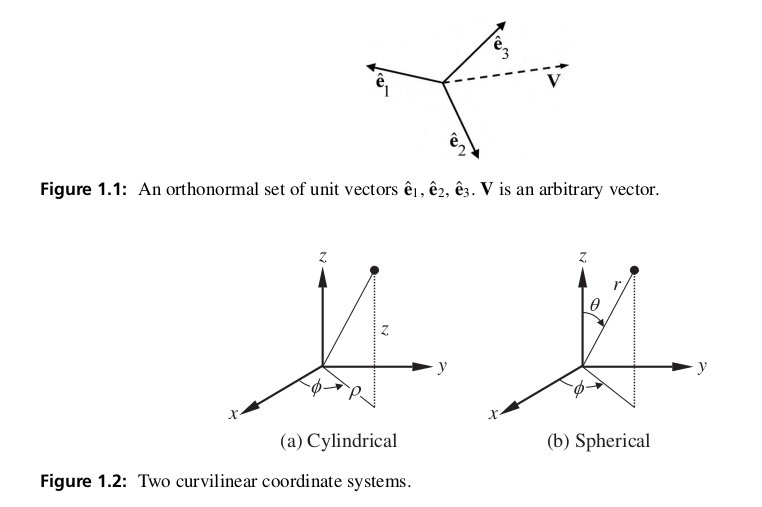
\includegraphics[width=0.7\linewidth]{exemplo_bases.png}

\end{figure}\end{frame}


% ============================================================
\begin{frame}{Base cartesiana ortonormal}
Escolha uma base ortonormal $\{\hat{\bm e}_1,\hat{\bm e}_2,\hat{\bm e}_3\}$ (frequentemente $\hat{\bm x},\hat{\bm y},\hat{\bm z}$).
\begin{equation}
\hat{\bm e}_i\cdot \hat{\bm e}_j=\delta_{ij}
\label{eq:ortonormal}
\end{equation}

\begin{equation}
\hat{\bm e}_1\times\hat{\bm e}_2=\hat{\bm e}_3,\quad
\hat{\bm e}_2\times\hat{\bm e}_3=\hat{\bm e}_1,\quad
\hat{\bm e}_3\times\hat{\bm e}_1=\hat{\bm e}_2
\label{eq:rhs}
\end{equation}

\begin{block}{Representação de $\bm V$}
\begin{equation}
\bm V = V_1\hat{\bm e}_1+V_2\hat{\bm e}_2+V_3\hat{\bm e}_3
\label{eq:Vdecomp}
\end{equation}
\end{block}
\end{frame}

% ============================================================
\begin{frame}{Como obter as componentes: demonstração}
Partimos de \eqref{eq:Vdecomp} e fazemos produto escalar com $\hat{\bm e}_k$:
\begin{equation}
\hat{\bm e}_k\cdot\bm V
=\hat{\bm e}_k\cdot\left(\sum_{i=1}^3 V_i\hat{\bm e}_i\right)
=\sum_{i=1}^3 V_i(\hat{\bm e}_k\cdot\hat{\bm e}_i)
=\sum_{i=1}^3 V_i\delta_{ki}
=V_k.
\label{eq:Vk_demo}
\end{equation}

Logo,
\begin{equation}
V_k=\hat{\bm e}_k\cdot \bm V.
\label{eq:Vk}
\end{equation}

\begin{alertblock}{Interpretação}
As componentes são \red{projeções} do vetor na base escolhida.
\end{alertblock}
\end{frame}

% ============================================================
\begin{frame}{Mudança de base: ideia essencial}
Considere duas bases ortonormais $\{\hat{\bm e}_i\}$ e $\{\hat{\bm e}'_i\}$.

Escreva o mesmo vetor nas duas bases:
\begin{equation}
\bm V=\sum_{i=1}^3 V_i\hat{\bm e}_i
=\sum_{i=1}^3 V'_i\hat{\bm e}'_i.
\label{eq:V_two_bases}
\end{equation}

Defina a matriz de mudança de base
\begin{equation}
R_{ij}=\hat{\bm e}'_i\cdot\hat{\bm e}_j.
\label{eq:Rij}
\end{equation}

Então, projetando \eqref{eq:V_two_bases} em $\hat{\bm e}'_i$:
\begin{equation}
V'_i=\hat{\bm e}'_i\cdot\bm V
=\sum_{j=1}^3 V_j(\hat{\bm e}'_i\cdot\hat{\bm e}_j)
=\sum_{j=1}^3 R_{ij}V_j.
\label{eq:Vprime_RV}
\end{equation}

\begin{block}{Resumo}
\red{Componentes transformam linearmente:} $V'_i=R_{ij}V_j$.
\end{block}
\end{frame}

% ============================================================
\begin{frame}{Sistemas de coordenadas: por que aparecem?}
\begin{block}{Três sistemas centrais}
\begin{itemize}
  \item Cartesiano $(x,y,z)$: geometria ``plana'' local, operadores simples.
  \item Cilíndrico $(\rho,\phi,z)$: simetria axial (fios, solenoides longos).
  \item Esférico $(r,\theta,\phi)$: simetria radial (carga puntiforme, ondas).
\end{itemize}
\end{block}

\begin{alertblock}{Cuidado}
Operadores diferenciais mudam de forma porque os vetores unitários \red{dependem da posição} em coordenadas curvilíneas.
\end{alertblock}
\end{frame}

% ============================================================
\begin{frame}{Cartesiano: posição e diferenciais}
Vetor posição:
\begin{equation}
\bm r=x\hat{\bm x}+y\hat{\bm y}+z\hat{\bm z}.
\label{eq:r_cart}
\end{equation}

Diferencial de deslocamento:
\begin{equation}
d\bm r=dx\,\hat{\bm x}+dy\,\hat{\bm y}+dz\,\hat{\bm z}.
\label{eq:dr_cart}
\end{equation}

Elemento de volume:
\begin{equation}
d^3r=dx\,dy\,dz.
\label{eq:d3_cart}
\end{equation}

\begin{block}{Nota}
Em cartesiano, os unitários são constantes: $\partial_x\hat{\bm x}=0$ etc.
\end{block}
\end{frame}

% ============================================================
\begin{frame}{Gradiente em cartesiano (definição + interpretação)}
Definição: para um escalar $\phi(\bm r)$, o gradiente é o vetor que satisfaz
\begin{equation}
d\phi = \nabla\phi\cdot d\bm r.
\label{eq:def_grad}
\end{equation}

Em cartesiano, usando \eqref{eq:dr_cart}:
\begin{equation}
d\phi=\pdv{\phi}{x}dx+\pdv{\phi}{y}dy+\pdv{\phi}{z}dz.
\label{eq:dphi_cart}
\end{equation}

Comparando \eqref{eq:def_grad} e \eqref{eq:dphi_cart}, obtemos:
\begin{equation}
\nabla = \hat{\bm x}\pdv{}{x}+\hat{\bm y}\pdv{}{y}+\hat{\bm z}\pdv{}{z}.
\label{eq:grad_cart}
\end{equation}

\begin{alertblock}{Interpretação}
$\nabla\phi$ aponta na direção de maior crescimento de $\phi$ e tem módulo igual à taxa máxima de variação por comprimento.
\end{alertblock}
\end{frame}

% ============================================================
\begin{frame}{Divergência e rotacional (cartesiano)}
Para um campo vetorial $\bm V=V_x\hat{\bm x}+V_y\hat{\bm y}+V_z\hat{\bm z}$:

\begin{equation}
\nabla\cdot\bm V=\pdv{V_x}{x}+\pdv{V_y}{y}+\pdv{V_z}{z}.
\label{eq:div_cart}
\end{equation}

\begin{equation}
\nabla\times\bm V=
\left(\pdv{V_z}{y}-\pdv{V_y}{z}\right)\hat{\bm x}
+\left(\pdv{V_x}{z}-\pdv{V_z}{x}\right)\hat{\bm y}
+\left(\pdv{V_y}{x}-\pdv{V_x}{y}\right)\hat{\bm z}.
\label{eq:curl_cart}
\end{equation}

\begin{block}{Laplaciano de escalar}
\begin{equation}
\nabla^2\phi=\pdv[2]{\phi}{x}+\pdv[2]{\phi}{y}+\pdv[2]{\phi}{z}.
\label{eq:lap_cart}
\end{equation}
\end{block}
\end{frame}

% ============================================================
\begin{frame}{Coordenadas Cilíndricas: transformação e base}
Transformações:
\begin{equation}
x=\rho\cos\phi,\quad y=\rho\sin\phi,\quad z=z.
\label{eq:cyl_transform}
\end{equation}

Unitários dependem de $\phi$:
\begin{equation}
\hat{\bm \rho}=\cos\phi\,\hat{\bm x}+\sin\phi\,\hat{\bm y},\quad
\hat{\bm \phi}=-\sin\phi\,\hat{\bm x}+\cos\phi\,\hat{\bm y},\quad
\hat{\bm z}=\hat{\bm z}.
\label{eq:unit_cyl}
\end{equation}

\begin{alertblock}{Consequência}
Como $\hat{\bm \rho}$ e $\hat{\bm \phi}$ mudam com $\phi$, derivadas exigem cuidado extra.
\end{alertblock}
\notas{pág. 1}
\end{frame}


\begin{frame}
    \begin{alertblock}{Observação}
Veja que $\hat{\bm \phi} = \frac{1}{\rho}\frac{\partial}{\partial\phi}$ e $\hat{\bm \rho} = \frac{\partial}{\partial\rho}$.
\end{alertblock}
\notas{pág. 2 e 3}
\end{frame}

% ============================================================
\begin{frame}{Cilíndricas: elemento de linha e volume (demonstração curta)}
Comece com \eqref{eq:cyl_transform} e diferencie:
\begin{equation}
dx=\cos\phi\,d\rho-\rho\sin\phi\,d\phi,\quad
dy=\sin\phi\,d\rho+\rho\cos\phi\,d\phi,\quad
dz=dz.
\label{eq:cyl_diff}
\end{equation}

Então
\begin{equation}
ds^2=dx^2+dy^2+dz^2=d\rho^2+\rho^2d\phi^2+dz^2.
\label{eq:ds2_cyl}
\end{equation}

Logo,
\begin{equation}
d\bm r=\hat{\bm\rho}\,d\rho+\hat{\bm\phi}\,\rho d\phi+\hat{\bm z}\,dz,
\label{eq:dr_cyl}
\end{equation}
e o elemento de volume:
\begin{equation}
d^3r=\rho\,d\rho\,d\phi\,dz.
\label{eq:d3_cyl}
\end{equation}
\end{frame}

% ============================================================
\begin{frame}{Operadores em cilíndricas (forma final)}
Para um escalar $\phi(\rho,\phi,z)$:
\begin{equation}
\nabla\phi=\hat{\bm\rho}\pdv{\phi}{\rho}
+\hat{\bm\phi}\frac{1}{\rho}\pdv{\phi}{\phi}
+\hat{\bm z}\pdv{\phi}{z}.
\label{eq:grad_cyl}
\end{equation}

Para $\bm V=V_\rho\hat{\bm\rho}+V_\phi\hat{\bm\phi}+V_z\hat{\bm z}$:
\begin{equation}
\nabla\cdot\bm V=\frac{1}{\rho}\pdv{}{\rho}\left(\rho V_\rho\right)
+\frac{1}{\rho}\pdv{V_\phi}{\phi}
+\pdv{V_z}{z}.
\label{eq:div_cyl}
\end{equation}

\begin{equation}
\nabla\times\bm V=
\left[\frac{1}{\rho}\pdv{V_z}{\phi}-\pdv{V_\phi}{z}\right]\hat{\bm\rho}
+\left[\pdv{V_\rho}{z}-\pdv{V_z}{\rho}\right]\hat{\bm\phi}
+\frac{1}{\rho}\left[\pdv{}{\rho}(\rho V_\phi)-\pdv{V_\rho}{\phi}\right]\hat{\bm z}.
\label{eq:curl_cyl}
\end{equation}
\notas{pág. 4}
\end{frame}

% ============================================================
\begin{frame}{Coordenadas Esféricas: transformação e elemento de volume}
Transformações:
\begin{equation}
x=r\sin\theta\cos\phi,\quad
y=r\sin\theta\sin\phi,\quad
z=r\cos\theta.
\label{eq:sph_transform}
\end{equation}

Elemento de linha (resultado padrão):
\begin{equation}
ds^2=dr^2+r^2d\theta^2+r^2\sin^2\theta\,d\phi^2.
\label{eq:ds2_sph}
\end{equation}

Elemento de volume:
\begin{equation}
d^3r=r^2\sin\theta\,dr\,d\theta\,d\phi.
\label{eq:d3_sph}
\end{equation}

\begin{block}{Uso típico}
Simetria radial em problemas eletrostáticos e radiação.
\end{block}
\notas{ pags 5,6,7 $\rightarrow$ vetores unitários}
\end{frame}

% ============================================================
\begin{frame}{Operadores em esféricas}
Para escalar $\phi(r,\theta,\phi)$:
\begin{equation}
\nabla\phi=\hat{\bm r}\pdv{\phi}{r}
+\hat{\bm\theta}\frac{1}{r}\pdv{\phi}{\theta}
+\hat{\bm\phi}\frac{1}{r\sin\theta}\pdv{\phi}{\phi}.
\label{eq:grad_sph}
\end{equation}

Para $\bm V=V_r\hat{\bm r}+V_\theta\hat{\bm\theta}+V_\phi\hat{\bm\phi}$:
\begin{equation}
\nabla\cdot\bm V=\frac{1}{r^2}\pdv{}{r}\left(r^2V_r\right)
+\frac{1}{r\sin\theta}\pdv{}{\theta}\left(\sin\theta\,V_\theta\right)
+\frac{1}{r\sin\theta}\pdv{V_\phi}{\phi}.
\label{eq:div_sph}
\end{equation}

\begin{equation}
\nabla^2\phi=\frac{1}{r^2}\pdv{}{r}\left(r^2\pdv{\phi}{r}\right)
+\frac{1}{r^2\sin\theta}\pdv{}{\theta}\left(\sin\theta\,\pdv{\phi}{\theta}\right)
+\frac{1}{r^2\sin^2\theta}\pdv[2]{\phi}{\phi}.
\label{eq:lap_sph}
\end{equation}
\notas{ pag 7}
\end{frame}



% ============================================================
\begin{frame}{Convenção de soma de Einstein}
\begin{block}{Regra}
Um índice repetido exatamente duas vezes em um termo implica soma automática:
$A_iB_i\equiv \sum_{i=1}^3 A_iB_i$.
\end{block}

Exemplos:
\begin{equation}
\bm V = V_k\hat{\bm e}_k
\label{eq:einstein_V}
\end{equation}
\begin{equation}
\bm V\cdot\bm F = V_kF_k.
\label{eq:einstein_dot}
\end{equation}

\begin{alertblock}{Cuidado}
O \red{intervalo} do índice deve estar claro pelo contexto (tipicamente $1,2,3$ em 3D cartesiano).
\end{alertblock}
\end{frame}


\begin{frame}{Índices Mudos e Índices Livres}

\textbf{Índices Mudos}

\begin{equation}
\vec{V} = V_k\,\hat{e}_k
\end{equation}

O índice \(k\) é chamado de \textbf{índice mudo}.  

Em qualquer equação, índices mudos podem ser trocados sem alterar o resultado:

\begin{equation}
V_k\,\hat{e}_k = V_j\,\hat{e}_j
\end{equation}

\end{frame}

\begin{frame}{Índices Mudos e Índices Livres}

\textbf{Índices Livres}

\begin{equation}
A_i = \sum_{j} R_{ij} B_j = R_{ij} B_j
\end{equation}

Aqui \(i\) é chamado de \textbf{índice livre}.

Em coordenadas cartesianas,
\[
i = x, y, z
\]
Logo, a equação acima representa na verdade 3 equações, para $A_x$, $A_y$ e $A_z$.

\begin{alertblock}{Atenção}
Em geral, \textbf{não se pode trocar índices livres}.
\end{alertblock}

\end{frame}
% ============================================================
\begin{frame}{Kronecker e Levi-Civita}
\begin{block}{Símbolos fundamentais}
\begin{equation}
\delta_{ij}=
\begin{cases}
1,& i=j,\\
0,& i\neq j,
\end{cases}
\label{eq:kronecker}
\end{equation}

\begin{equation}
\varepsilon_{ijk}=
\begin{cases}
+1,& (ijk)\ \text{par de }(123),\\
-1,& (ijk)\ \text{ímpar de }(123),\\
0,& \text{se algum índice repete.}
\end{cases}
\label{eq:levicivita}
\end{equation}
\end{block}

\begin{alertblock}{Leitura geométrica}
$\delta_{ij}$ ``seleciona'' componentes; $\varepsilon_{ijk}$ codifica orientação e produtos vetoriais.
\end{alertblock}
\end{frame}

% ============================================================
\begin{frame}{Produto vetorial via Levi-Civita (demonstração)}
Defina o produto vetorial componente a componente:
\begin{equation}
(\bm A\times \bm B)_i=\varepsilon_{ijk}A_jB_k.
\label{eq:cross_eps}
\end{equation}

\red{Verificação rápida} para $i=1$:
\begin{equation}
(\bm A\times\bm B)_1=\varepsilon_{123}A_2B_3+\varepsilon_{132}A_3B_2
= A_2B_3-A_3B_2,
\label{eq:cross_i1}
\end{equation}

\end{frame}

% ============================================================
\begin{frame}{Identidade-chave: contração de Levi-Civita}
Identidade padrão:
\begin{equation}
\varepsilon_{ijk}\varepsilon_{imn}=\delta_{jm}\delta_{kn}-\delta_{jn}\delta_{km}.
\label{eq:eps_eps}
\end{equation}

\red{Uso imediato}: simplificar expressões com duplo produto vetorial e provar identidades.

\begin{alertblock}{Por que isso aparece em EM?}
Porque $\nabla\times(\nabla\times\bm A)$, tensores e ondas eletromagnéticas ficam naturais nesse formalismo.
\end{alertblock}

\notas{ exemplo em pag 8.}

\end{frame}

% ============================================================
\begin{frame}{Exemplo: prova de $\nabla\cdot(\nabla\times\bm g)=0$}
Escreva o rotacional em componentes:
\begin{equation}
(\nabla\times\bm g)_i=\varepsilon_{ijk}\partial_j g_k.
\label{eq:curl_comp}
\end{equation}

Então a divergência:
\begin{equation}
\nabla\cdot(\nabla\times\bm g)=\partial_i(\nabla\times\bm g)_i
=\partial_i(\varepsilon_{ijk}\partial_j g_k)
=\varepsilon_{ijk}\partial_i\partial_j g_k.
\label{eq:divcurl_1}
\end{equation}

Como $\partial_i\partial_j=\partial_j\partial_i$ (derivadas parciais comutam para campos suaves),
o termo $\partial_i\partial_j g_k$ é simétrico em $(i,j)$, enquanto $\varepsilon_{ijk}$ é antissimétrico em $(i,j)$.
Logo, a contração é zero:
\begin{equation}
\varepsilon_{ijk}\partial_i\partial_j g_k=0.
\label{eq:divcurl_2}
\end{equation}
\end{frame}


\begin{frame}{Contração entre Tensores Simétricos e Antissimétricos}

\textbf{Definições}

Tensor simétrico:
\begin{equation}
S_{ij} = S_{ji}
\end{equation}

Tensor antissimétrico:
\begin{equation}
A_{ij} = -A_{ji}
\end{equation}

\end{frame}

\begin{frame}

\textbf{Contração}

\begin{equation}
S_{ij}A_{ij}
\end{equation}

Trocando os índices mudos \(i \leftrightarrow j\):

\begin{equation}
S_{ij}A_{ij} = S_{ji}A_{ji}
\end{equation}

Usando as propriedades de simetria:

\begin{equation}
S_{ji}A_{ji} = S_{ij}(-A_{ij}) = -S_{ij}A_{ij}
\end{equation}

Logo,

\begin{equation}
S_{ij}A_{ij} = -S_{ij}A_{ij}
\label{eq:symantisym}
\end{equation}

\begin{alertblock}{Resultado}
\begin{equation}
S_{ij}A_{ij} = 0
\end{equation}
Sempre que a contração ocorre nos índices onde os tensores são
simétrico e antissimétrico.
\end{alertblock}

\end{frame}
% ================================================% ============================================================
\begin{frame}{Exercícios}
\begin{block}{Prove as identidades vetoriais abaixo}
Mostre, usando notação indicial (Kronecker/Levi-Civita) ou regras do operador $\nabla$,
que as identidades a seguir são válidas (assuma campos suficientemente suaves):
\end{block}

\vspace{-0.2cm}
\small
\begin{align}
\nabla\cdot\nabla \varphi &= \nabla^2\varphi,
\tag{1}\label{eq:ex_id_1}\\[0.15cm]
\nabla\cdot(\nabla\times \bm F) &= 0,
\tag{2}\label{eq:ex_id_2}\\[0.15cm]
\nabla\times(\nabla \varphi) &= 0,
\tag{3}\label{eq:ex_id_3}\\[0.15cm]
\nabla\times(\nabla\times \bm F) &= \nabla(\nabla\cdot \bm F)-\nabla^2\bm F,
\tag{4}\label{eq:ex_id_4}\\[0.15cm]
\nabla(\varphi\psi) &= (\nabla\varphi)\psi+\varphi\,\nabla\psi,
\tag{5}\label{eq:ex_id_5}
\end{align}
\normalsize
\end{frame}

% ============================================================
\begin{frame}{Exercícios (continuação)}
\vspace{-0.2cm}
\small
\begin{align}
\nabla(\bm F\cdot \bm G) &= (\bm F\cdot\nabla)\bm G+\bm F\times(\nabla\times\bm G)
+(\bm G\cdot\nabla)\bm F+\bm G\times(\nabla\times\bm F),
\tag{6}\label{eq:ex_id_6}\\[0.15cm]
\nabla\cdot(\varphi\,\bm F) &= (\nabla\varphi)\cdot\bm F+\varphi\,(\nabla\cdot\bm F),
\tag{7}\label{eq:ex_id_7}\\[0.15cm]
\nabla\cdot(\bm F\times \bm G) &= (\nabla\times\bm F)\cdot\bm G-(\nabla\times\bm G)\cdot\bm F,
\tag{8}\label{eq:ex_id_8}\\[0.15cm]
\nabla\times(\varphi\,\bm F) &= (\nabla\varphi)\times\bm F+\varphi\,(\nabla\times\bm F),
\tag{9}\label{eq:ex_id_9}\\[0.15cm]
\nabla\times(\bm F\times \bm G) &= (\nabla\cdot\bm G)\bm F-(\nabla\cdot\bm F)\bm G
+(\bm G\cdot\nabla)\bm F-(\bm F\cdot\nabla)\bm G.
\tag{10}\label{eq:ex_id_10}
\end{align}
\normalsize
\end{frame}

% ============================================================
\begin{frame}{Identidade vetorial: $\bm a\times(\bm b\times\bm c)$}
Queremos provar:
\begin{equation}
\bm a\times(\bm b\times\bm c)=\bm b(\bm a\cdot\bm c)-\bm c(\bm a\cdot\bm b).
\label{eq:triple_product}
\end{equation}

Em componentes:
\begin{equation}
\left[\bm a\times(\bm b\times\bm c)\right]_i
=\varepsilon_{ijk}a_j(\bm b\times\bm c)_k
=\varepsilon_{ijk}a_j\varepsilon_{kmn}b_m c_n.
\label{eq:triple_1}
\end{equation}

Use \eqref{eq:eps_eps}:
\begin{equation}
\varepsilon_{ijk}\varepsilon_{kmn}
=\delta_{im}\delta_{jn}-\delta_{in}\delta_{jm}.
\label{eq:eps_contract}
\end{equation}

Substituindo em \eqref{eq:triple_1}:
\begin{equation}
\left[\bm a\times(\bm b\times\bm c)\right]_i
=(\delta_{im}\delta_{jn}-\delta_{in}\delta_{jm})a_j b_m c_n
=b_i(a_j c_j)-c_i(a_j b_j),
\label{eq:triple_2}
\end{equation}
ou seja,
\begin{equation}
\left[\bm a\times(\bm b\times\bm c)\right]_i
=b_i(\bm a\cdot\bm c)-c_i(\bm a\cdot\bm b).
\label{eq:triple_3}
\end{equation}

Isso implica \eqref{eq:triple_product}.
\end{frame}

% ============================================================
% (ADICIONADO) PÁGINA DE TÍTULO — 1.3
\begin{frame}[plain]
\centering
\vfill
{\Huge\blue{1.3 Derivadas}}
\vfill
\end{frame}

% ============================================================
\begin{frame}{1.3 Derivadas — Funções de $\bm r$ e $|\bm r|$}
\begin{block}{Definições}
O vetor posição é
\[
\bm r = r\,\hat{\bm r}, \qquad r=\sqrt{x^2+y^2+z^2}.
\]
Se $f(r)$ é uma função escalar, definimos $f'(r)=df/dr$.
\end{block}

\begin{block}{Identidades básicas}
\begin{equation}
\nabla r = \hat{\bm r},
\qquad
\nabla \times \bm r = 0,
\tag{1.58}
\label{eq:grad_r}
\end{equation}

\begin{equation}
\nabla f = f'(r)\,\hat{\bm r},
\qquad
\nabla^2 f = \frac{(r^2 f')'}{r^2}.
\tag{1.59}
\label{eq:gradf_lapf}
\end{equation}
\end{block}
\notas{ pag 13, 14}
\end{frame}

% ============================================================
\begin{frame}{1.3 Derivadas — Divergência e rotacional}
\begin{block}{Campo do tipo $f(r)\bm r$}
\begin{equation}
\nabla\cdot\big(f(r)\bm r\big)
=
\frac{(r^3 f)'}{r^2},
\qquad
\nabla\times\big(f(r)\bm r\big)=0.
\tag{1.60}
\label{eq:div_fr}
\end{equation}
\end{block}

\begin{block}{Campo vetorial $\bm g(r)$}
Se $\bm g(r)$ é um campo vetorial e $\bm c$ um vetor constante:
\begin{equation}
\nabla\cdot \bm g = \bm g'\cdot\hat{\bm r},
\qquad
\nabla\times \bm g = \hat{\bm r}\times \bm g'.
\tag{1.61}
\label{eq:grad_g}
\end{equation}

\begin{equation}
(\bm g\cdot\nabla)\bm r = \bm g,
\qquad
(\bm r\cdot\nabla)\bm g = r\,\bm g'.
\tag{1.62}
\label{eq:rgrad_g}
\end{equation}
\end{block}
\notas{ pag 15}
\end{frame}

% ============================================================
\begin{frame}{1.3 Derivadas — Produtos vetoriais}
\begin{block}{Produto escalar e vetorial}
\begin{equation}
\nabla(\bm r\cdot\bm g)
=
\bm g+\frac{(\bm r\cdot\bm g')\bm r}{r},
\qquad
\nabla\cdot(\bm g\times\bm r)=0.
\tag{1.63}
\label{eq:grad_rg}
\end{equation}
\end{block}

\begin{block}{Identidades finais}
\begin{equation}
\nabla\times(\bm g\times\bm r)
=
2\bm g+r\,\bm g'
-\frac{(\bm r\cdot\bm g')\bm r}{r},
\qquad
\nabla(\bm c\cdot\bm r)=\bm c.
\tag{1.64}
\label{eq:curl_gr}
\end{equation}
\end{block}

\begin{alertblock}{Observação}
Essas identidades são especialmente úteis em problemas com
\red{simetria esférica}, comuns em eletrostática e gravitação.
\end{alertblock}
\end{frame}
 


% ============================================================
\begin{frame}{1.3.2 Funções de $\bm r-\bm r'$}
\begin{block}{Definição}
Defina o vetor deslocamento
\[
\bm R = \bm r - \bm r'
= (x-x')\hat{\bm x}+(y-y')\hat{\bm y}+(z-z')\hat{\bm z},
\qquad
R = |\bm R|.
\]
Se $f(R)$ é uma função escalar e $\bm g(R)$ um campo vetorial,
com derivada $f'(R)=df/dR$.
\end{block}

\begin{block}{Identidades fundamentais}
\begin{equation}
\nabla f(R) = f'(R)\,\hat{\bm R},
\qquad
\nabla\cdot \bm g(R) = \bm g'(R)\cdot \hat{\bm R},
\qquad
\nabla\times \bm g(R) = \hat{\bm R}\times \bm g'(R).
\tag{1.65}
\label{eq:R_identities}
\end{equation}
\end{block}
\notas{ pag 16}
\end{frame}

% ============================================================
\begin{frame}{1.3.2 Derivadas em $\bm r$ e $\bm r'$}
\begin{block}{Operadores diferenciais}
Os operadores gradiente com respeito a $\bm r$ e $\bm r'$ são
\begin{equation}
\nabla = \hat{\bm x}\pdv{}{x}
+ \hat{\bm y}\pdv{}{y}
+ \hat{\bm z}\pdv{}{z},
\qquad
\nabla' = \hat{\bm x}\pdv{}{x'}
+ \hat{\bm y}\pdv{}{y'}
+ \hat{\bm z}\pdv{}{z'}.
\tag{1.66}
\label{eq:grad_gradprime}
\end{equation}
\end{block}

\begin{block}{Relação chave}
Como $\bm R=\bm r-\bm r'$, segue diretamente que
\begin{equation}
\nabla' f(R) = -\,\nabla f(R).
\tag{1.67}
\label{eq:gradprime_R}
\end{equation}
\end{block}

\begin{alertblock}{Importância física}
Essas relações são essenciais na formulação de \red{potenciais},
funções de Green e campos gerados por distribuições contínuas de carga.
\end{alertblock}
\notas{ pag 18}
\end{frame}


% ============================================================
\begin{frame}{1.3.3 A Derivada Convectiva}
\begin{block}{Ideia física}
Se $\phi(\bm r,t)$ é uma função escalar do espaço e do tempo:
\begin{itemize}
  \item um observador fixo em $\bm r$ mede a taxa de variação $\partial\phi/\partial t$;
  \item um observador que se move ao longo de uma trajetória $\bm r(t)$,
  com velocidade $\bm v(t)=\dot{\bm r}(t)$, mede uma taxa de variação diferente.
\end{itemize}
\end{block}

\begin{block}{Definição}
A taxa de variação de $\phi$ ao longo da trajetória é a \blue{derivada convectiva}:
\begin{equation}
\frac{d\phi}{dt}
=
\pdv{\phi}{t}
+\frac{dx}{dt}\pdv{\phi}{x}
+\frac{dy}{dt}\pdv{\phi}{y}
+\frac{dz}{dt}\pdv{\phi}{z}
=
\pdv{\phi}{t}
+(\bm v\cdot\nabla)\phi.
\tag{1.68}
\label{eq:convective_scalar}
\end{equation}
\end{block}
\notas{ pag 19}
\end{frame}

\begin{frame}
\begin{block}{Campo vetorial}
Para um campo vetorial $\bm g(\bm r,t)$, a derivada convectiva é
\begin{equation}
\frac{d\bm g}{dt}
=
\pdv{\bm g}{t}
+(\bm v\cdot\nabla)\bm g.
\tag{1.69}
\label{eq:convective_vector}
\end{equation}
\end{block}

\begin{alertblock}{Contexto}
Essa derivada é central em hidrodinâmica, MHD e na descrição do movimento de cargas em campos eletromagnéticos.
\end{alertblock}
\end{frame}


% ============================================================
\begin{frame}{1.3.4 Teorema de Taylor — uma dimensão}
\begin{block}{Forma padrão}
O teorema de Taylor em uma dimensão é
\begin{equation}
f(x)
=
f(a)
+(x-a)\left.\dv{f}{x}\right|_{x=a}
+\frac{1}{2!}(x-a)^2\left.\dv[2]{f}{x}\right|_{x=a}
+\cdots .
\tag{1.70}
\label{eq:taylor_1d}
\end{equation}
\end{block}

\begin{block}{Forma deslocada}
Fazendo $x\to x+\epsilon$ e $a\to x$, obtemos
\begin{equation}
f(x+\epsilon)
=
f(x)
+\epsilon\dv{f}{x}
+\frac{1}{2!}\epsilon^2\dv[2]{f}{x}
+\cdots .
\tag{1.71}
\label{eq:taylor_shift}
\end{equation}
\end{block}
\notas{ pag 20-21}
\end{frame}

% ============================================================
\begin{frame}{1.3.4 Teorema de Taylor — operador exponencial}
\begin{block}{Forma operacional}
A expansão de Taylor pode ser escrita de forma compacta como
\begin{equation}
f(x+\epsilon)
=
\left[
1
+\epsilon\dv{}{x}
+\frac{1}{2!}\left(\epsilon\dv{}{x}\right)^2
+\cdots
\right] f(x)
=
\exp\!\left(\epsilon\dv{}{x}\right) f(x).
\tag{1.72}
\label{eq:taylor_exp_1d}
\end{equation}
\end{block}

\begin{alertblock}{Interpretação}
O operador $\exp\!\left(\epsilon\dv{}{x}\right)$ atua como um
\red{operador de translação} ao longo do eixo $x$.
\end{alertblock}
\end{frame}

% ============================================================
\begin{frame}{1.3.4 Teorema de Taylor — várias variáveis}
\begin{block}{Generalização para três variáveis}
Para $f(x,y,z)$:
\begin{equation}
f(x+\epsilon_x,y+\epsilon_y,z+\epsilon_z)
=
\exp\!\left(\epsilon_x\pdv{}{x}\right)
\exp\!\left(\epsilon_y\pdv{}{y}\right)
\exp\!\left(\epsilon_z\pdv{}{z}\right)
f(x,y,z).
\tag{1.73}
\label{eq:taylor_xyz}
\end{equation}
\end{block}

\begin{block}{Forma vetorial}
Definindo $\bm\epsilon=(\epsilon_x,\epsilon_y,\epsilon_z)$:
\begin{equation}
f(\bm r+\bm\epsilon)
=
\exp(\bm\epsilon\cdot\nabla)\,f(\bm r)
=
\left[
1
+\bm\epsilon\cdot\nabla
+\frac{1}{2!}(\bm\epsilon\cdot\nabla)^2
+\cdots
\right] f(\bm r).
\tag{1.74}
\label{eq:taylor_vector}
\end{equation}
\end{block}

\begin{alertblock}{Importância em EM}
Essa forma é essencial na derivação de expansões multipolares,
potenciais e funções de Green.
\end{alertblock}
\end{frame}

% ============================================================
% (ADICIONADO) PÁGINA DE TÍTULO — 1.4
\begin{frame}[plain]
\centering
\vfill
{\Huge\blue{1.4 Integrais}}
\vfill
\end{frame}

% ============================================================
\begin{frame}{1.4 Integrais — 1.4.1 Determinante Jacobiano}
\begin{block}{Ideia central}
O determinante da matriz Jacobiana relaciona \blue{elementos de volume}
quando realizamos uma mudança de variáveis em uma integral.
\end{block}

Se $\bm x$ e $\bm y$ são vetores em $\mathbb{R}^N$, associados a dois sistemas
de coordenadas diferentes, os elementos de volume satisfazem
\begin{equation}
d^N x = \left| \mathbf J(\bm x,\bm y) \right|\, d^N y,
\tag{1.75}
\label{eq:jacobian_general}
\end{equation}
\end{frame}


\begin{frame}

onde $\mathbf J$ é a matriz Jacobiana
\[
\mathbf J(\bm x,\bm y)
=
\begin{vmatrix}
\dfrac{\partial x_1}{\partial y_1} &
\dfrac{\partial x_1}{\partial y_2} & \cdots &
\dfrac{\partial x_1}{\partial y_N} \\[0.6em]
\dfrac{\partial x_2}{\partial y_1} &
\dfrac{\partial x_2}{\partial y_2} & \cdots &
\dfrac{\partial x_2}{\partial y_N} \\
\vdots & \vdots & \ddots & \vdots \\
\dfrac{\partial x_N}{\partial y_1} &
\dfrac{\partial x_N}{\partial y_2} & \cdots &
\dfrac{\partial x_N}{\partial y_N}
\end{vmatrix}.
\]
\notas{Exemplo polar pag 24}
\end{frame}

% ============================================================
\begin{frame}{1.4.1 Exemplo — cartesiano $\rightarrow$ esférico}
\begin{block}{Transformação}
Considere a mudança de variáveis
\[
x=r\sin\theta\cos\phi,\quad
y=r\sin\theta\sin\phi,\quad
z=r\cos\theta.
\]
\end{block}

O determinante Jacobiano é
\begin{equation}
\left|\mathbf J\right|
=
\left|
\pdv{(x,y,z)}{(r,\theta,\phi)}
\right|
=
r^2\sin\theta.
\label{eq:jacobian_spherical}
\end{equation}

\begin{block}{Elemento de volume}
Portanto, o elemento de volume transforma-se como
\begin{equation}
d^3x = r^2\sin\theta\,dr\,d\theta\,d\phi.
\label{eq:d3_spherical}
\end{equation}
\end{block}
\end{frame}

\begin{frame}

\begin{alertblock}{Importância em EM}
Jacobianos aparecem sistematicamente em integrais de carga,
fluxos e na aplicação dos teoremas de Gauss e Stokes.
\end{alertblock}
\end{frame}

% ============================================================
\begin{frame}{1.4.2 O Teorema da Divergência}
\begin{block}{Enunciado}
Seja $\bm F(\bm r)$ um campo vetorial definido em um volume $V$,
limitado por uma superfície fechada $S$ com normal externa
$\hat{\bm n}$. Se $d\bm S = dS\,\hat{\bm n}$, então:
\end{block}

\begin{equation}
\int_V d^3 r\, \nabla\cdot \bm F
=
\int_S dS\, \bm F\cdot\hat{\bm n}.
\tag{1.76}
\label{eq:divergence_theorem}
\end{equation}

\begin{alertblock}{Leitura física}
O fluxo total de $\bm F$ que sai de $V$ é igual à soma das fontes
(contidas no volume).
\end{alertblock}
\end{frame}

% ============================================================
\begin{frame}{Consequência I — identidade escalar}
\begin{block}{Escolha especial do campo}
Seja $\bm c$ um vetor constante arbitrário e escolha
\[
\bm F(\bm r)=\bm c\,\psi(\bm r).
\]
\end{block}

Substituindo em \eqref{eq:divergence_theorem} e usando
$\nabla\cdot(\bm c\,\psi)=\bm c\cdot\nabla\psi$, obtemos:
\begin{equation}
\int_V d^3 r\, \nabla\psi
=
\int_S dS\, \psi\,\hat{\bm n}.
\tag{1.77}
\label{eq:grad_identity}
\end{equation}

\begin{alertblock}{Interpretação}
O gradiente integrado no volume é determinado apenas
pelos valores de $\psi$ na fronteira.
\end{alertblock}
\notas{ pag 26}
\end{frame}

% ============================================================
\begin{frame}{Consequência II — identidade vetorial}
\begin{block}{Nova escolha do campo}
Escolha agora
\[
\bm F(\bm r)=\bm A(\bm r)\times\bm c,
\]
onde $\bm c$ é um vetor constante.
\end{block}

Usando $\nabla\cdot(\bm A\times\bm c)
=\bm c\cdot(\nabla\times\bm A)$ e aplicando
\eqref{eq:divergence_theorem}, resulta:
\begin{equation}
\int_V d^3 r\, \nabla\times\bm A
=
\int_S dS\, \hat{\bm n}\times\bm A.
\tag{1.78}
\label{eq:curl_identity}
\end{equation}

\begin{alertblock}{Importância}
Esta identidade é fundamental para:
\begin{itemize}
  \item condições de contorno em eletromagnetismo;
  \item formulações integrais das equações de Maxwell.
\end{itemize}
\end{alertblock}
\notas{pag 27}
\end{frame}


% ============================================================
\begin{frame}{1.4.3 Identidades de Green — motivação}
\begin{block}{Ideia central}
As identidades de Green são consequências diretas do
\blue{Teorema da Divergência} e conectam:
\begin{itemize}
  \item operadores diferenciais no volume;
  \item valores dos campos na superfície.
\end{itemize}
\end{block}

\begin{alertblock}{Por que são importantes?}
Elas são a base matemática de:
\begin{itemize}
  \item problemas de valor de contorno;
  \item funções de Green;
  \item unicidade de soluções em eletrostática.
\end{itemize}
\end{alertblock}
\end{frame}

% ============================================================
\begin{frame}{Primeira identidade de Green}
\begin{block}{Escolha do campo}
Escolha no Teorema da Divergência:
\[
\bm F(\bm r)=\phi(\bm r)\,\nabla\psi(\bm r).
\]
\end{block}

Aplicando \eqref{eq:divergence_theorem}, obtemos a \textbf{Primeira Identidade de Green}:
\begin{equation}
\int_V d^3 r\,
\big[
\phi\,\nabla^2\psi
+
\nabla\phi\cdot\nabla\psi
\big]
=
\int_S dS\,
\phi\,\nabla\psi\cdot\hat{\bm n}.
\tag{1.79}
\label{eq:green_first}
\end{equation}

\begin{alertblock}{Leitura}
Derivadas de $\psi$ no volume $\leftrightarrow$
fluxo ponderado por $\phi$ na fronteira.
\end{alertblock}
\notas{pag 29}
\end{frame}

% ============================================================
\begin{frame}{Segunda identidade de Green}
\begin{block}{Construção}
Troque $\phi \leftrightarrow \psi$ em \eqref{eq:green_first}
e subtraia as duas expressões. Obtemos a \textbf{Segunda Identidade Green}
\end{block}

\begin{equation}
\int_V d^3 r\,
\big[
\phi\,\nabla^2\psi
-
\psi\,\nabla^2\phi
\big]
=
\int_S dS\,
\big[
\phi\,\nabla\psi
-
\psi\,\nabla\phi
\big]\cdot\hat{\bm n}.
\tag{1.80}
\label{eq:green_second}
\end{equation}

\begin{alertblock}{Mensagem-chave}
Esta identidade elimina os termos de gradiente cruzados $\nabla\phi\!\cdot\!\nabla\psi$, restando apenas os Laplacianos $\nabla^2\psi$ e $\nabla^2\phi$. 
\end{alertblock}
\end{frame}

\begin{frame}{Por que o Laplaciano é tão importante?}
\small

\begin{block}{\textbf{Ideia central}}
Na física de campos, o \textbf{Laplaciano de um potencial} está diretamente ligado à
\textbf{densidade de fontes}. Em eletrostática, por exemplo:
\begin{equation}
\nabla^2 \phi = -\frac{\rho}{\varepsilon_0}
\label{eq:poisson}
\end{equation}
\end{block}

\vspace{0.2cm}

\begin{alertblock}{\textbf{Por que isso é tão poderoso?}}
A segunda identidade de Green
\begin{equation}
\int_V d^3r\,\left(\phi \nabla^2\psi - \psi \nabla^2\phi\right)
=
\int_S dS\,\left(\phi \nabla\psi - \psi \nabla\phi\right)\cdot\hat{n}
\label{eq:green2}
\end{equation}
permite \textbf{trocar informação de volume} (\emph{fontes}) por
\textbf{informação de superfície} (\emph{contorno}).
\end{alertblock}

\end{frame}

\begin{frame}


\begin{exampleblock}{\textbf{Mensagem física}}
\begin{itemize}
    \item Os termos com \(\nabla^2\phi\) e \(\nabla^2\psi\) têm \textbf{significado físico direto}:
    eles representam as \textbf{fontes do campo}.
    \item Já os termos de gradiente cruzado, como \(\nabla\phi\cdot\nabla\psi\), são
    matematicamente úteis, mas menos transparentes fisicamente.
    \item A identidade de Green reorganiza a expressão de modo a destacar justamente
    \textbf{o papel das fontes e das condições de contorno}.
\end{itemize}
\end{exampleblock}

\end{frame}

% ============================================================
\begin{frame}{Identidade de Green — versão vetorial (I)}
\begin{block}{Escolha vetorial}
Escolha agora
\[
\bm F=\bm P\times(\nabla\times\bm Q)
\]
e use a identidade
$\nabla\cdot(\bm A\times\bm B)
=\bm B\cdot(\nabla\times\bm A)-\bm A\cdot(\nabla\times\bm B)$.
\end{block}

\begin{equation}
\int_V d^3 r\,
\Big[
\nabla\times\bm P\cdot\nabla\times\bm Q
-
\bm P\cdot\nabla\times\nabla\times\bm Q
\Big]
=
\int_S dS\,
\hat{\bm n}\cdot
(\bm P\times\nabla\times\bm Q).
\tag{1.81}
\label{eq:green_vector_first}
\end{equation}
\notas{pag 31}
\end{frame}

% ============================================================
\begin{frame}{Identidade de Green — versão vetorial (II)}
\begin{block}{Segunda identidade vetorial}
Troque $\bm P \leftrightarrow \bm Q$ em \eqref{eq:green_vector_first}
e subtraia as duas expressões.
\end{block}

\begin{equation}
\int_V d^3 r\,
\Big[
\bm Q\cdot\nabla\times\nabla\times\bm P
-
\bm P\cdot\nabla\times\nabla\times\bm Q
\Big]
=
\int_S dS\,
\hat{\bm n}\cdot
\big[
\bm P\times\nabla\times\bm Q
-
\bm Q\times\nabla\times\bm P
\big].
\tag{1.82}
\label{eq:green_vector_second}
\end{equation}

\begin{alertblock}{Interpretação}
Versão vetorial da segunda identidade de Green.
\end{alertblock}
\end{frame}

% ============================================================
    \begin{frame}{Exemplo}
\begin{block}{Tipo de problema (não vamos resolver ainda)}
O potencial eletrostático $\phi$ satisfaz:
\[
\nabla^2\phi(\bm r)=-\frac{\rho(\bm r)}{\varepsilon_0}.
\]
Queremos determinar $\phi$ dentro de um volume $V$
a partir da carga e das condições de contorno.
\end{block}

Escolha na segunda identidade de Green:
\[
\psi(\bm r)=\frac{1}{|\bm r-\bm r'|},
\qquad
\nabla^2\psi=-4\pi\delta(\bm r-\bm r').
\]

Resulta a representação integral:
\begin{equation}
\phi(\bm r)
=
\frac{1}{4\pi\varepsilon_0}
\int_V d^3 r'\,
\frac{\rho(\bm r')}{|\bm r-\bm r'|}
+\text{(termos de contorno)}.
\end{equation}

\end{frame}

\begin{frame}

\begin{alertblock}{Conclusão}
As identidades de Green conectam
\red{equações diferenciais locais}
a
\blue{soluções integrais globais}
— exatamente o que precisamos em eletrodinâmica.
\end{alertblock}
\end{frame}


% ============================================================
\begin{frame}{1.4.4 O Teorema de Stokes — enunciado}
\begin{block}{Situação geométrica}
Seja $\bm F(\bm r)$ um campo vetorial definido
sobre uma superfície aberta $S$, limitada por uma
curva fechada $C$.
\end{block}

Se $d\bm S=\hat{\bm n}\,dS$ é o elemento de área orientado
e $d\bm \ell$ é o elemento de linha ao longo de $C$,
então o Teorema de Stokes afirma:
\begin{equation}
\int_S d\bm S\cdot(\nabla\times\bm F)
=
\oint_C d\bm \ell\cdot\bm F.
\tag{1.83}
\label{eq:stokes}
\end{equation}

\begin{alertblock}{Leitura física}
A circulação de $\bm F$ ao longo da borda
é determinada pelo rotacional de $\bm F$
no interior da superfície.
\end{alertblock}
\notas{pag 33}
\end{frame}

\begin{frame}

\begin{center}
    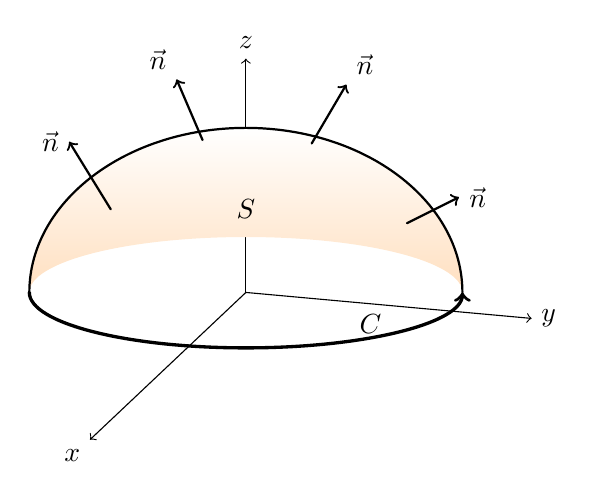
\begin{tikzpicture}[scale=2.2,line cap=round,line join=round]

% parâmetros da calota
\def\a{1.25}   % semi-eixo horizontal
\def\b{0.95}   % semi-eixo vertical

%---------------------------
% eixos
%---------------------------
\draw[->] (0,0) -- (-0.9,-0.85) node[below left] {$x$};
\draw[->] (0,0) -- (1.65,-0.15) node[right] {$y$};
\draw[->] (0,0) -- (0,1.35) node[above] {$z$};

%---------------------------
% preenchimento da calota superior
%---------------------------
\shade[left color=blue!65,right color=orange!25,top color=white!85]
(-\a,0) arc[start angle=180,end angle=0,x radius=\a,y radius=\b]
-- (\a,0)
arc[start angle=0,end angle=180,x radius=\a,y radius=0.32]
-- cycle;

%---------------------------
% contorno visível da superfície S
%---------------------------
\draw[thick]
(-\a,0) arc[start angle=180,end angle=0,x radius=\a,y radius=\b];

% contorno C
\draw[very thick,->]
(-\a,0) arc[start angle=180,end angle=360,x radius=\a,y radius=0.32];
\node at (0.72,-0.18) {$C$};

%---------------------------
% vetores normais
%---------------------------
\draw[->,thick] (-0.78,0.48) -- (-1.02,0.87) node[left] {$\vec n$};
\draw[->,thick] (-0.25,0.88) -- (-0.4,1.23) node[above left] {$\vec n$};
\draw[->,thick] (0.38,0.86) -- (0.58,1.20) node[above right] {$\vec n$};
\draw[->,thick] (0.93,0.40) -- (1.23,0.55) node[right] {$\vec n$};

%---------------------------
% rótulo da superfície
%---------------------------
\node at (0,0.48) {$S$};

\end{tikzpicture}
\end{center}
\end{frame}

% ============================================================
\begin{frame}{Orientação e regra da mão direita}
\begin{block}{Orientação consistente}
A curva $C$ deve ser percorrida no sentido
determinado pela \blue{regra da mão direita}:
\end{block}

\begin{itemize}
  \item o polegar aponta na direção de $d\bm S$;
  \item os dedos indicam o sentido positivo de integração em $C$.
\end{itemize}

\begin{alertblock}{Cuidado conceitual}
Trocar a orientação de $S$ inverte o sinal da integral de linha.
\end{alertblock}

\begin{block}{Analogia}
Stokes é a versão bidimensional do Teorema da Divergência.
\end{block}
\end{frame}

% ============================================================
\begin{frame}{Consequência I — campo do tipo gradiente}
\begin{block}{Escolha especial do campo}
Escolha
\[
\bm F = \nabla\psi.
\]
\end{block}

Como $\nabla\times(\nabla\psi)=0$, o Teorema de Stokes
implica:
\begin{equation}
\oint_C d\bm \ell\cdot\nabla\psi = 0.
\tag{1.84}
\label{eq:grad_circulation}
\end{equation}

\begin{alertblock}{Interpretação}
Campos gradientes são \red{irrotacionais}:
a circulação ao longo de qualquer curva fechada é nula.
\end{alertblock}
\end{frame}


\begin{frame}{Campos Gradientes e Conservação}

\textbf{Interpretação física }
\begin{itemize}
    \item O trabalho ao longo de qualquer curva fechada é zero
    \item O trabalho entre dois pontos \textbf{não depende do caminho}
\end{itemize}

\vspace{0.4cm}

\textbf{Definição de campo conservativo}
\begin{itemize}
    \item Um campo é conservativo se:
    \begin{equation}
    \label{eq:conservativo}
    \oint_C \mathbf{F}\cdot d\mathbf{l} = 0
    \end{equation}
    \item Ou seja, podemos escrevê-lo como o gradiente de um potencial escalar:
    \begin{equation}
    \label{eq:potencial}
    \mathbf{F} = -\nabla U
    \end{equation}
\end{itemize}

\vspace{0.4cm}
\end{frame}

\begin{frame}
\textbf{Conexão com conservação}
\begin{itemize}
    \item Existe uma energia potencial \(U\) tal que:
    \begin{equation}
    \label{eq:trabalho}
    W_{A \to B} = U(A) - U(B)
    \end{equation}
    \item A energia mecânica se conserva
    \item Não há “perda” ao dar uma volta completa
\end{itemize}

\vspace{0.4cm}

\textbf{Resumo conceitual}
\begin{equation}
\label{eq:resumo}
\mathbf{F} = \nabla \psi 
\;\Rightarrow\; 
\nabla \times \mathbf{F} = 0 
\;\Rightarrow\; 
\oint \mathbf{F}\cdot d\mathbf{l} = 0 
\;\Rightarrow\; 
\text{campo conservativo}
\end{equation}

\vspace{0.2cm}

\textbf{Intuição}
\begin{itemize}
    \item Campo com rotação (redemoinho): \textbf{não conservativo}
    \item Campo gradiente (descida de montanha): \textbf{conservativo}
\end{itemize}

\end{frame}
% ============================================================
\begin{frame}{Consequência II — escolha vetorial}
\begin{block}{Nova escolha}
Escolha
\[
\bm F=\bm A\times\bm c,
\]
onde $\bm c$ é um vetor constante.
\end{block}

Usando identidades vetoriais e aplicando \eqref{eq:stokes},
obtemos:
\begin{equation}
\oint_C d\boldsymbol{\ell} \times \mathbf{A}
=
\int_S dS_k\,\nabla A_k
-
\int_S d\mathbf{S}\,(\nabla \cdot \mathbf{A}).
\tag{1.85}
\end{equation}

\begin{alertblock}{Uso}
Esta forma aparece em manipulações integrais
de campos vetoriais em eletrodinâmica.
\end{alertblock}
\notas{pag 36}
\end{frame}

% ============================================================
\begin{frame}{Exemplo — Lei de Faraday}
\begin{block}{Contexto físico}
Na eletrodinâmica clássica,
a Lei de Faraday na forma diferencial é:
\[
\nabla\times\bm E = -\pdv{\bm B}{t}.
\]
\end{block}

Aplicando o Teorema de Stokes \eqref{eq:stokes}:
\begin{equation}
\oint_C \bm E\cdot d\bm \ell
=
-\,\pdv{}{t}
\int_S \bm B\cdot d\bm S.
\end{equation}

\end{frame}

\begin{frame}

\begin{alertblock}{Conclusão}
O Teorema de Stokes conecta:
\begin{itemize}
  \item o \red{rotacional local} do campo elétrico
  \item à \blue{força eletromotriz} induzida ao longo de um circuito.
\end{itemize}
Sem Stokes, a passagem entre as formas
integral e diferencial das equações de Maxwell
não seria possível.
\end{alertblock}
\end{frame}


% ============================================================
\begin{frame}{1.4.5 Derivada temporal de integrais de Superfície — Regra de Leibniz}
\begin{block}{Integral unidimensional com limites móveis}
Se $b(x,t)$ é uma função suave e os limites dependem do tempo,
a regra de Leibniz afirma:
\end{block}

\begin{equation}
\dv{}{t}\int_{x_1(t)}^{x_2(t)} dx\, b(x,t)
=
b(x_2,t)\dv{x_2}{t}
-
b(x_1,t)\dv{x_1}{t}
+
\int_{x_1(t)}^{x_2(t)} dx\, \pdv{b}{t}.
\tag{1.86}
\label{eq:leibniz}
\end{equation}

\begin{alertblock}{Ideia-chave}
A variação temporal vem de:
\begin{itemize}
  \item mudanças do integrando;
  \item movimento das fronteiras.
\end{itemize}
\end{alertblock}
\notas{pag 38-40}
\end{frame}

% ============================================================
\begin{frame}{Generalização para superfícies móveis}

\begin{figure}
    \centering
    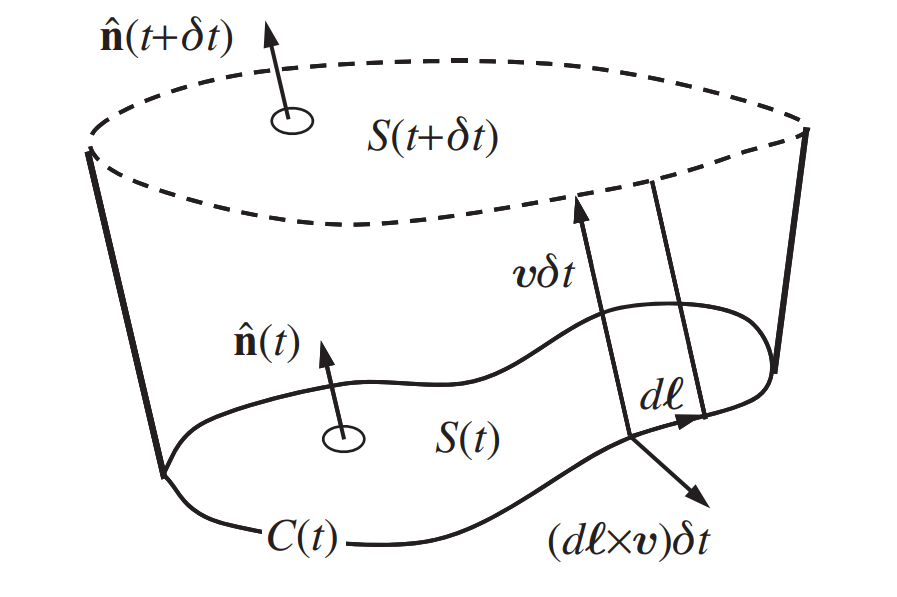
\includegraphics[width=0.5\linewidth]{sup_movel.png}
    \caption{Figure 1.3: A surface $S(t)$ [bounded by the solid curve labeled $C(t)$] changes to the surface $S(t + \delta t)$ (dashed
curve) because each element of surface moves by an amount $\bm{\mathcal{v}}\,\delta t$.}
\end{figure}
\notas{pag 41}
\end{frame}


\begin{frame}{Generalização para superfícies móveis}
\begin{block}{Contexto físico}
Em eletrodinâmica, integramos campos sobre
\blue{superfícies que se movem no espaço}.
\end{block}

Considere uma superfície $S(t)$ cujos elementos de área
movem-se com velocidade $\bm v(\bm r,t)$.
O resultado geral para o fluxo magnético é:
\begin{equation}
\dv{}{t}\int_{S(t)} d\bm S\cdot\bm B
=
\int_{S(t)} d\bm S\cdot
\Big[
\bm v(\nabla\cdot\bm B)
-
\nabla\times(\bm v\times\bm B)
+
\pdv{\bm B}{t}
\Big].
\tag{1.87}
\label{eq:flux_time_derivative}
\end{equation}

\begin{alertblock}{Importância}
Esta expressão é essencial para a formulação correta
da Lei de Faraday.
\end{alertblock}
\end{frame}

% ============================================================
\begin{frame}{Estratégia da demonstração}
\begin{block}{Variação infinitesimal do fluxo}
Começamos avaliando a variação:
\end{block}

\begin{equation}
\delta\!\left[\int \bm B\cdot d\bm S\right]
=
\int \delta\bm B\cdot d\bm S
+
\int \bm B\cdot\delta(\hat{\bm n}dS).
\tag{1.88}
\label{eq:flux_variation}
\end{equation}

\begin{itemize}
  \item primeiro termo: variação temporal do campo $\bm B$;
  \item segundo termo: deformação e movimento da superfície.
\end{itemize}
\end{frame}

% ============================================================
\begin{frame}{Separação dos termos temporais}
Dividindo \eqref{eq:flux_variation} por $\delta t$, obtemos:
\begin{equation}
\dv{}{t}\int \bm B\cdot d\bm S
=
\int \pdv{\bm B}{t}\cdot d\bm S
+
\frac{1}{\delta t}\int \bm B\cdot\delta(\hat{\bm n}dS).
\tag{1.89}
\label{eq:flux_time_split}
\end{equation}

\begin{alertblock}{Observação}
O primeiro termo já aparece explicitamente em \eqref{eq:flux_time_derivative};
o foco passa a ser o segundo.
\end{alertblock}
\end{frame}

% ============================================================
\begin{frame}{Construção geométrica auxiliar}
\begin{block}{Volume infinitesimal}
Considere o volume $V$ limitado por:
\begin{itemize}
  \item a superfície $S(t)$;
  \item a superfície $S(t+\delta t)$;
  \item a superfície lateral em forma de fita.
\end{itemize}
\end{block}

Aplicando o Teorema da Divergência:
\begin{equation}
\int_V d^3 r\, \nabla\cdot\bm B
=
\int_{S(t+\delta t)} \bm B\cdot\hat{\bm n}dS
-
\int_{S(t)} \bm B\cdot\hat{\bm n}dS
+
\oint_{C(t)} \bm B\cdot(d\bm\ell\times\bm v\,\delta t).
\tag{1.90}
\label{eq:aux_volume}
\end{equation}

\begin{alertblock}{Sinal}
O sinal negativo decorre da normal externa ao volume $V$.
\end{alertblock}
\end{frame}

% ============================================================
\begin{frame}{Redução do termo geométrico}
Usando:
\[
d^3 r = \hat{\bm n}\cdot\bm v\,\delta t\, dS,
\qquad
\bm B\cdot(d\bm\ell\times\bm v)=d\bm\ell\cdot(\bm v\times\bm B),
\]
a Eq.~\eqref{eq:aux_volume} leva a:
\begin{equation}
\delta t\int_{S(t)} d\bm S\,\bm v(\nabla\cdot\bm B)
=
\int_{S(t)} \bm B\cdot\delta(\hat{\bm n}dS)
+
\delta t\oint_{C(t)} d\bm\ell\cdot(\bm v\times\bm B).
\tag{1.91}
\label{eq:geom_identity}
\end{equation}
\notas{pag 43}
\end{frame}

% ============================================================
\begin{frame}{Uso do Teorema de Stokes e resultado final}
Aplicando o Teorema de Stokes à integral de linha em \eqref{eq:geom_identity}:
\begin{equation}
\int_{S(t)} \bm B\cdot\delta(\hat{\bm n}dS)
=
\delta t\int_{S(t)} dS\,\bm v(\nabla\cdot\bm B)
-
\delta t\int_{S(t)} dS\,\nabla\times(\bm v\times\bm B).
\tag{1.92}
\label{eq:stokes_step}
\end{equation}

Substituindo \eqref{eq:stokes_step} em \eqref{eq:flux_time_split},
recuperamos exatamente a Eq.~\eqref{eq:flux_time_derivative}.

\begin{alertblock}{Mensagem final}
A derivada temporal do fluxo combina:
\begin{itemize}
  \item variação explícita do campo;
  \item movimento e deformação da superfície;
  \item topologia da borda (via Stokes).
\end{itemize}
\end{alertblock}
\end{frame}
 

% ============================================================
% (ADICIONADO) PÁGINAS DE TÍTULO PARA TÓPICOS AINDA NÃO INCLUÍDOS
\begin{frame}[plain]
\centering
\vfill
{\Huge\blue{1.5 Funções Generalizadas}}
\vfill
\end{frame}

\begin{frame}{1.5.1 The Delta Function in One Dimension}

\begin{block}{Definição (ação de filtragem)}
A função delta unidimensional $\delta(x)$ é definida pela sua ação
sobre uma função teste suave $f(x)$:
\end{block}

\begin{equation}
\int_{-\infty}^{\infty} dx\, f(x)\,\delta(x-x') = f(x').
\tag{1.93}
\end{equation}

\begin{block}{Definição informal equivalente}
\begin{equation}
\delta(x)=0 \;\; (x\neq 0),
\qquad
\int_{-\infty}^{\infty} dx\,\delta(x)=1.
\tag{1.94}
\end{equation}
\end{block}

\begin{alertblock}{Observação dimensional}
Se $x$ tem dimensão de comprimento, então $\delta(x)$ tem dimensão
de inverso de comprimento.
\end{alertblock}
\notas{pag 45}
\end{frame}

\begin{frame}{Delta como limite de sequências}

A função delta pode ser entendida como o limite de funções cada vez
mais concentradas em $x=0$:

\begin{equation}
\delta(x)=\lim_{m\to\infty}\frac{\sin(mx)}{\pi x},
\tag{1.95}
\end{equation}

\begin{equation}
\delta(x)=\lim_{m\to\infty}\frac{m}{\sqrt{\pi}}\,e^{-m^2x^2},
\tag{1.96}
\end{equation}

\begin{equation}
\delta(x)=\lim_{\epsilon\to 0}\frac{\epsilon/\pi}{x^2+\epsilon^2}.
\tag{1.97}
\end{equation}

\begin{block}{Ideia-chave}
Todas essas sequências satisfazem a propriedade de filtragem (1.93).
\end{block}

\end{frame}

\begin{frame}
Pode-se provar o exemplo (1.95) pelo uso da propriedade de filtragem:

\begin{equation}
\int_{-\infty}^{\infty} dx\, f(x)\,\delta(x) = f(0).
\end{equation}

Substituindo (1.95) na equação acima, temos que provar que é verdade que:

\begin{equation}
\delta(x)=\lim_{m\to\infty} \int_{-\infty}^{\infty} dx\, f(x)\,\frac{\sin(mx)}{\pi x} = f(0)
\end{equation}

    
\end{frame}

\begin{frame}
   O Plot mostra o que acontece com o integrando de (67) nos limites $m\rightarrow 0$ e $m\rightarrow \infty$
   \begin{figure}
       \centering
       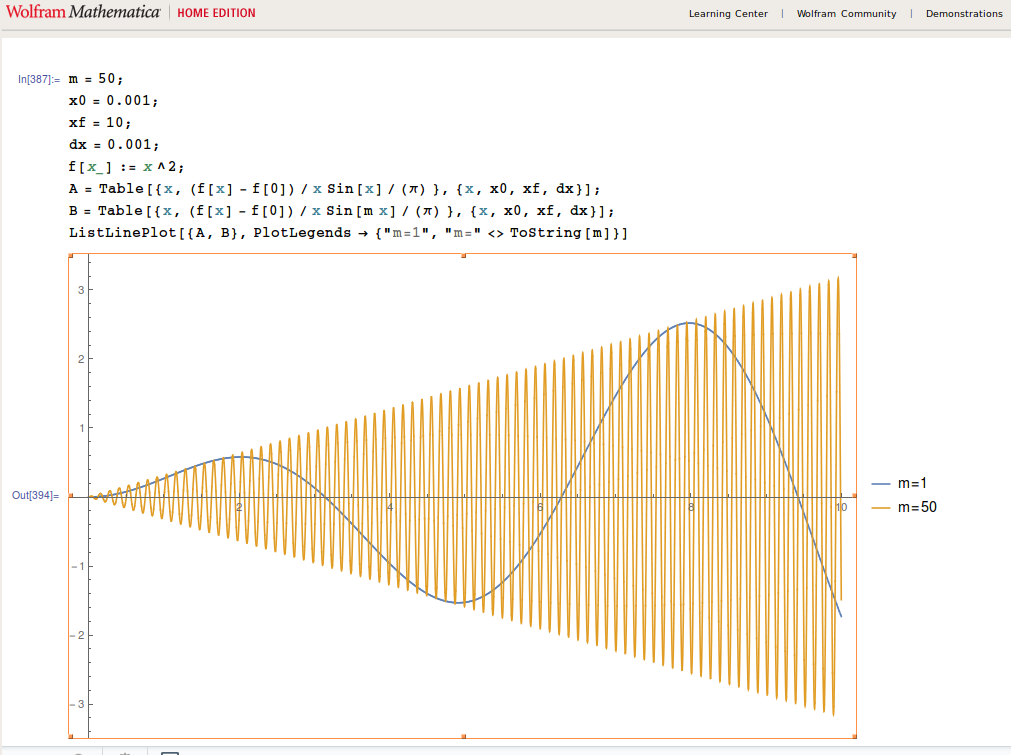
\includegraphics[width=0.6\linewidth]{Limite2.png}

   \end{figure}
\end{frame}

%------------------------------------------------
\begin{frame}{1.5.2 O Valor Principal}

{\color{myblue}
O valor principal de Cauchy é uma função generalizada definida por sua ação sob uma integral com uma função arbitrária $f(x)$:
}

\vspace{0.4cm}

\begin{equation}
\mathcal{P}\!\!\int_{-\infty}^{\infty}
\frac{f(x)}{x-x_0}\,dx
=
\lim_{\epsilon\to 0}
\left[
\int_{-\infty}^{x_0-\epsilon}
\frac{f(x)}{x-x_0}\,dx
+
\int_{x_0+\epsilon}^{\infty}
\frac{f(x)}{x-x_0}\,dx
\right]
\tag{1.104}
\end{equation}

\begin{alertblock}{Interpretação}
Remove-se um intervalo \textbf{simétrico} ao redor da singularidade.
\end{alertblock}

\end{frame}

%------------------------------------------------
\begin{frame}{Exemplo}

A integral comum diverge:

\[
\int_{-1}^{1} \frac{dx}{x}
\]

Mas o valor principal é:

\[
\mathcal{P}\int_{-1}^{1} \frac{dx}{x}
=
\lim_{\epsilon\to 0}
\left(
\int_{-1}^{\epsilon}\frac{dx}{x}
+
\int_{\epsilon}^{1}\frac{dx}{x}
\right)
\]

\begin{block}{Resultado}
As divergências se cancelam e o valor é zero.
\end{block}
\notas{pag 48}
\end{frame}

%------------------------------------------------
\begin{frame}{Convergência como Distribuição}

{\color{myred}
Existem funções que não convergem ponto a ponto,
mas convergem dentro de uma integral.
}

\vspace{0.4cm}

Exemplo:

\[
\delta_m(x)=\frac{\sin(mx)}{\pi x}
\]

\[
\lim_{m\to\infty}
\int \delta_m(x)\,\varphi(x)\,dx
=
\varphi(0)
\]

\begin{alertblock}{Conclusão}
Não convergem como função, mas convergem como distribuição.
\end{alertblock}
\notas{pag 49}
\end{frame}

%------------------------------------------------
\begin{frame}{Exemplo Fundamental da Física}

Quando $\epsilon \to 0$:

\[
\frac{1}{x \pm i\epsilon}
\]

\begin{itemize}
\item Não converge como função
\item Converge como distribuição
\end{itemize}

\begin{tcolorbox}[colback=blue!5,colframe=myblue]
\[
\lim_{\epsilon\to 0^+}
\frac{1}{x\pm i\epsilon}
=
\mathcal{P}\frac{1}{x}
\mp i\pi\delta(x)
\tag{1.105}
\]
\end{tcolorbox}

\end{frame}

%------------------------------------------------
\begin{frame}{Demonstração: Identidade Algébrica}

Partimos da identidade:

\begin{equation}
\frac{1}{x-x_0 \pm i\epsilon}
=
\frac{x-x_0}{(x-x_0)^2+\epsilon^2}
\mp i
\frac{\epsilon}{(x-x_0)^2+\epsilon^2}
\tag{1.106}
\end{equation}

Separando:

\begin{itemize}
\item Parte real
\item Parte imaginária
\end{itemize}
\notas{pag 51}
\end{frame}

%------------------------------------------------
\begin{frame}{Parte Imaginária}

Usamos:

\[
\delta(x-x_0)
=
\lim_{\epsilon\to 0^+}
\frac{1}{\pi}
\frac{\epsilon}{(x-x_0)^2+\epsilon^2}
\]

Logo:

\[
\lim_{\epsilon\to 0}
\int
f(x)
\frac{\epsilon}{(x-x_0)^2+\epsilon^2}
dx
=
\pi f(x_0)
\]

\begin{alertblock}{Resultado}
Parte imaginária $\to \mp i\pi f(x_0)$
\end{alertblock}

\end{frame}

%------------------------------------------------
\begin{frame}{Parte Real: Symmetrical Cutoff}

Observe:

\[
\frac{x-x_0}{(x-x_0)^2+\epsilon^2}
=
\frac{1}{x-x_0}
\cdot
\frac{(x-x_0)^2}{(x-x_0)^2+\epsilon^2}
\]

{\color{mypurple}
Quando $|x-x_0|\gg \epsilon$, o fator tende a 1.
}

\vspace{0.3cm}

{\color{mypurple}
Perto de $x=x_0$, a função é ímpar e sua integral se cancela.
}

\end{frame}

%------------------------------------------------
\begin{frame}{Gráfico da Parte Real}

\begin{center}
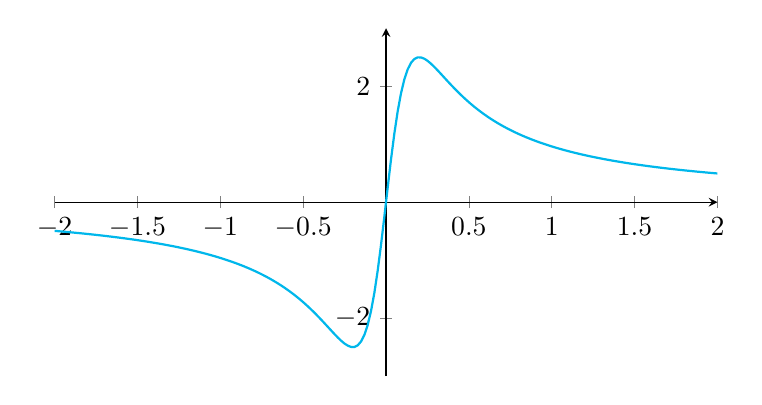
\begin{tikzpicture}
\begin{axis}[
width=10cm,
height=6cm,
axis lines=middle,
xmin=-2, xmax=2,
ymin=-3, ymax=3,
samples=200,
domain=-2:2
]
\addplot[myblue, thick] {(x)/(x^2+0.2^2)};
\end{axis}
\end{tikzpicture}
\end{center}

Função ímpar $\Rightarrow$ cancelamento simétrico.

\end{frame}

%------------------------------------------------
\begin{frame}{Resultado Final}

\[
\lim_{\epsilon\to 0^+}
\int
\frac{f(x)}{x-x_0 \pm i\epsilon}\,dx
=
\mathcal{P}
\int
\frac{f(x)}{x-x_0}\,dx
\mp i\pi f(x_0)
\]

\begin{tcolorbox}[colback=blue!5,colframe=myblue]
\[
\lim_{\epsilon\to 0}
\frac{1}{x-x_0 \pm i\epsilon}
=
\mathcal{P}\frac{1}{x-x_0}
\mp i\pi\delta(x-x_0)
\tag{1.105}
\]
\end{tcolorbox}

\end{frame}




\begin{frame}{Plemelj Formula}

\begin{block}{Identidade Fundamental}
\begin{equation}
\lim_{\epsilon\to 0}
\frac{1}{x-x_0 \pm i\epsilon}
=
\mathcal{P}\frac{1}{x-x_0}
\mp i\pi \delta(x-x_0).
\tag{1.105}
\end{equation}
\end{block}

\begin{block}{Interpretação}
A igualdade é simbólica: ganha significado quando multiplicamos
por uma função teste $f(x)$ e integramos sobre $x$.
\end{block}

\end{frame}

\begin{frame}{Estrutura da Identidade}

A identidade algébrica é:

\begin{equation}
\frac{1}{x-x_0 \pm i\epsilon}
=
\frac{x-x_0}{(x-x_0)^2+\epsilon^2}
\mp
i\,\frac{\epsilon}{(x-x_0)^2+\epsilon^2}.
\tag{1.106}
\end{equation}

\begin{block}{Interpretação Física}
\begin{itemize}
\item A parte real gera o valor principal
      (corte simétrico da singularidade).
\item A parte imaginária gera a função delta,
      via limite da forma Lorentziana (Eq. 1.97).
\end{itemize}
\end{block}

\end{frame}

\begin{frame}{Aplicações e Filosofia da Fórmula de Plemelj}

\begin{block}{A Fórmula}
\[
\lim_{\epsilon\to 0}
\frac{1}{x-x_0 \pm i\epsilon}
=
\mathcal{P}\frac{1}{x-x_0}
\mp i\pi \delta(x-x_0).
\]
\end{block}


\begin{block}{Filosofia}
\begin{itemize}
\item Singularidades reais são regularizadas deslocando o polo para o plano complexo.
\item O deslocamento $\pm i\epsilon$ codifica informação causal.
\item No limite, a parte real produz o \textbf{valor principal} (simetria).
\item A parte imaginária produz a \textbf{delta} (contribuição localizada).
\item A identidade é válida no sentido de distribuições.
\end{itemize}
\end{block}

\end{frame}

\begin{frame}
    
\begin{block}{Principais Aplicações}
\begin{itemize}
\item Transformadas de Fourier com polos reais.
\item Relações de dispersão (Kramers–Kronig).
\item Funções de Green e propagadores (prescrição causal).
\item Teoria quântica de campos (prescrição de Feynman).
\item Óptica e resposta linear (parte real vs parte imaginária).
\end{itemize}
\end{block}

\begin{alertblock}{Ideia Central}
A fórmula separa uma singularidade em duas contribuições:
uma distribuída (valor principal) e outra localizada (delta).
\end{alertblock}

\end{frame}


%------------------------------------------------
\begin{frame}{1.5.3 A Função Degrau}

A função degrau de Heaviside $\Theta(x)$ é definida por

\begin{equation}
\Theta(x)=
\begin{cases}
0, & x<0, \\
1, & x>0.
\end{cases}
\tag{1.107}
\end{equation}

\vspace{0.4cm}

A função delta é a derivada da função theta:

\begin{equation}
\frac{d\Theta(x)}{dx}=\delta(x).
\tag{1.108}
\end{equation}

\begin{tcolorbox}[colback=blue!5,colframe=blue]
$\delta(x)$ mede a descontinuidade de $\Theta(x)$.
\end{tcolorbox}

\end{frame}

%------------------------------------------------
\begin{frame}{Representação Integral de $\Theta(x)$}

Uma representação útil é

\begin{equation}
\Theta(x)
=
\lim_{\epsilon\to 0}
\frac{i}{2\pi}
\int_{-\infty}^{\infty}
\frac{dk}{k+i\epsilon}
e^{-ikx}.
\tag{1.109}
\end{equation}

\begin{itemize}
\item A prescrição $+i\epsilon$ impõe causalidade.
\item A descontinuidade em $x=0$ surge da estrutura de polos.
\end{itemize}
\notas{pag. 58}
636\end{frame}

%------------------------------------------------
\begin{frame}{A Função Sinal}

A função sinal $\mathrm{sgn}(x)$ é definida por

\begin{equation}
\mathrm{sgn}(x)
=
\frac{d}{dx}|x|
=
\begin{cases}
-1, & x<0, \\
1, & x>0.
\end{cases}
\tag{1.110}
\end{equation}

Uma representação conveniente é

\begin{equation}
\mathrm{sgn}(x)
=
-1
+
2\int_{-\infty}^{x}\delta(y)\,dy.
\tag{1.111}
\end{equation}

\begin{tcolorbox}[colback=blue!5,colframe=blue]
$\mathrm{sgn}(x)$ é a integral da função delta.
\end{tcolorbox}

\end{frame}


%------------------------------------------------

%------------------------------------------------
\begin{frame}{1.5.4 A Função Delta em Três Dimensões}

Definição via função teste:

\begin{equation}
\int_V d^3r\, f(\mathbf r)\delta(\mathbf r-\mathbf r')
=
\begin{cases}
f(\mathbf r'), & \mathbf r' \in V, \\
0, & \mathbf r' \notin V.
\end{cases}
\tag{1.112}
\end{equation}

Definição menos formal:

\begin{equation}
\delta(\mathbf r)=0 \;\; (\mathbf r\neq 0),
\quad
\int_V d^3r\,\delta(\mathbf r)
=
\begin{cases}
1, & \mathbf r=0\in V,\\
0, & \mathbf r=0\notin V.
\end{cases}
\tag{1.113}
\end{equation}

\end{frame}

%------------------------------------------------
\begin{frame}{Forma Cartesiana e Coordenadas Curvilíneas}

Em coordenadas cartesianas:

\begin{equation}
\delta(\mathbf r)=\delta(x)\delta(y)\delta(z).
\tag{1.114}
\end{equation}

Em coordenadas cilíndricas e esféricas:

\begin{equation}
\delta(\mathbf r-\mathbf r')
=
\frac{\delta(\rho-\rho')\delta(\phi-\phi')\delta(z-z')}{\rho}
=
\frac{\delta(r-r')\delta(\theta-\theta')\delta(\phi-\phi')}{r^2\sin\theta}.
\tag{1.115}
\end{equation}

\end{frame}

%------------------------------------------------
\begin{frame}{Caso Especial Radial}

Para $\mathbf r'=0$, definimos a delta radial:

\begin{equation}
\int_0^\infty dr\, \delta(r)=1.
\tag{1.116}
\end{equation}

\begin{tcolorbox}[colback=blue!5,colframe=blue]
A delta tridimensional tem dimensão de inverso de volume.
\end{tcolorbox}

\end{frame}

%------------------------------------------------
\begin{frame}{Transformação de Coordenadas}

Se $x_0$ e $y_0$ representam o mesmo ponto:

\begin{equation}
\int d^N x\, \delta(x-x_0)
=
\int d^N y\, \delta(y-y_0)
\tag{1.117}
\end{equation}

Usando o Jacobiano:

\begin{equation}
\delta(x-x_0)
=
\frac{1}{|J(x,y)|}
\delta(y-y_0).
\tag{1.118}
\end{equation}

\end{frame}

%------------------------------------------------
\begin{frame}{1.5.5 Identidades Úteis}

Representação de Fourier:

\begin{equation}
\delta(\mathbf r-\mathbf r')
=
\frac{1}{(2\pi)^3}
\int d^3k\, e^{i\mathbf k\cdot(\mathbf r-\mathbf r')}.
\tag{1.119}
\end{equation}

Integração sobre superfície:

\begin{equation}
\int d^3r\, f(r)\delta[g(r)]
=
\int_S dS \frac{f(r_S)}{|\nabla g(r_S)|}.
\tag{1.120}
\end{equation}

\end{frame}

%------------------------------------------------
\begin{frame}{Laplaciano de $1/r$}

\begin{equation}
\nabla^2 \frac{1}{|\mathbf r-\mathbf r'|}
=
-4\pi \delta(\mathbf r-\mathbf r').
\tag{1.121}
\end{equation}

Segunda derivada:

\begin{equation}
\frac{\partial^2}{\partial r_k \partial r_m}
\frac{1}{r}
=
\frac{3r_k r_m - r^2\delta_{km}}{r^5}
-
\frac{4\pi}{3}\delta_{km}\delta(\mathbf r).
\tag{1.122}
\end{equation}

\end{frame}

%------------------------------------------------
\begin{frame}{Exemplo 1.5: Prova via Teorema da Divergência}

Para $r\neq 0$:

\[
\nabla^2 \frac{1}{r}=0.
\]

Integrando sobre uma pequena esfera:

\[
\int_V d^3r\, \nabla^2 \frac{1}{r}
=
\int_S dS\, \left(-\frac{\hat r}{r^2}\right)
=
-4\pi.
\]

\begin{tcolorbox}[colback=blue!5,colframe=blue]
Logo,
\[
\nabla^2 \frac{1}{r}
=
-4\pi\delta(\mathbf r).
\]
\end{tcolorbox}

\end{frame}

%------------------------------------------------

\begin{frame}[plain]
\centering
\vfill
{\Huge\blue{1.6 Análise de Fourrier}}
\vfill
\end{frame}



%------------------------------------------------
\begin{frame}{1.6 Análise de Fourier — Série de Fourier}

Toda função periódica $f(x+L)=f(x)$ possui representação em série de Fourier:

\begin{equation}
f(x)=\sum_{m=-\infty}^{\infty}
\hat f_m e^{i2\pi m x/L}.
\tag{1.123}
\end{equation}

Os coeficientes são dados por

\begin{equation}
\hat f_m=
\frac{1}{L}
\int_0^L dx\, f(x)e^{-i2\pi m x/L}.
\tag{1.124}
\end{equation}

\end{frame}

%------------------------------------------------
\begin{frame}{Funções Não Periódicas — Transformada de Fourier}

Para funções não periódicas, a soma torna-se uma integral:

\begin{equation}
f(x)=
\frac{1}{2\pi}
\int_{-\infty}^{\infty}
dk\, \hat f(k)e^{ikx}.
\tag{1.125}
\end{equation}

\begin{equation}
\hat f(k)=
\int_{-\infty}^{\infty}
dx\, f(x)e^{-ikx}.
\tag{1.126}
\end{equation}

\end{frame}

%------------------------------------------------
\begin{frame}{Funções Reais}

Se $f(x)$ é real, então:

\begin{equation}
f(x)=f^*(x)
\quad \Rightarrow \quad
\hat f(k)=\hat f^*(-k).
\tag{1.127}
\end{equation}

\begin{tcolorbox}[colback=blue!5,colframe=blue]
A transformada de uma função real possui simetria hermitiana.
\end{tcolorbox}

\end{frame}

%------------------------------------------------
\begin{frame}{Domínio do Tempo}

No domínio temporal, convenciona-se escrever:

\begin{equation}
g(t)=
\frac{1}{2\pi}
\int_{-\infty}^{\infty}
d\omega\, \hat g(\omega)e^{-i\omega t},
\end{equation}

\begin{equation}
\hat g(\omega)=
\int_{-\infty}^{\infty}
dt\, g(t)e^{i\omega t}.
\tag{1.128}
\end{equation}

\end{frame}

%------------------------------------------------
\begin{frame}{Transformada de Fourier em 4D}

Para uma função $f(\mathbf r,t)$:

\begin{equation}
f(\mathbf r,t)=
\frac{1}{(2\pi)^4}
\int d^3k
\int_{-\infty}^{\infty}
d\omega\,
\hat f(\mathbf k|\omega)
e^{i(\mathbf k\cdot \mathbf r-\omega t)}.
\tag{1.129}
\end{equation}

\end{frame}

%------------------------------------------------
\begin{frame}{Transformada Inversa 4D}

\begin{equation}
\hat f(\mathbf k|\omega)=
\int d^3r
\int_{-\infty}^{\infty}
dt\,
f(\mathbf r,t)
e^{-i(\mathbf k\cdot \mathbf r-\omega t)}.
\tag{1.130}
\end{equation}

\begin{tcolorbox}[colback=blue!5,colframe=blue]
Convenção simétrica: todos os fatores $(2\pi)$ aparecem na transformada inversa.
\end{tcolorbox}

\end{frame}

%------------------------------------------------


%------------------------------------------------
\begin{frame}{1.6.1 Teorema de Parseval}

\begin{equation}
\int_{-\infty}^{\infty} dt\, g_1^*(t) g_2(t)
=
\frac{1}{2\pi}
\int_{-\infty}^{\infty}
d\omega\,
\hat g_1^*(\omega)\hat g_2(\omega).
\tag{1.131}
\end{equation}

\begin{tcolorbox}[colback=blue!5,colframe=blue]
O teorema de Parseval afirma que o produto interno de duas funções
é preservado na transformada de Fourier.
\end{tcolorbox}

\end{frame}

%------------------------------------------------
\begin{frame}{Ideia da Prova}

A prova segue substituindo a transformada inversa

\[
g(t)=\frac{1}{2\pi}
\int d\omega\,\hat g(\omega)e^{-i\omega t}
\]

na equação de Parseval e utilizando a representação integral
da função delta.

\begin{tcolorbox}[colback=blue!5,colframe=blue]
A ortogonalidade das exponenciais complexas gera a função delta.
\end{tcolorbox}

\end{frame}

%------------------------------------------------
\begin{frame}{1.6.2 Teorema da Convolução}

Define-se a convolução de $f(t)$ e $g(t)$ como

\begin{equation}
h(t)=
\int_{-\infty}^{\infty}
dt'\,
f(t-t')g(t').
\tag{1.132}
\end{equation}

\begin{tcolorbox}[colback=blue!5,colframe=blue]
A convolução mede como uma função ``filtra'' ou
``suaviza'' outra.
\end{tcolorbox}

\end{frame}

%------------------------------------------------
\begin{frame}{Teorema da Convolução}

O teorema afirma que

\begin{equation}
\hat h(\omega)=\hat f(\omega)\hat g(\omega).
\tag{1.133}
\end{equation}

\begin{tcolorbox}[colback=blue!5,colframe=blue]
Convolução no domínio do tempo
corresponde a multiplicação no domínio de frequências.
\end{tcolorbox}

\end{frame}

%------------------------------------------------
\begin{frame}{Início da Prova}

Substituímos as transformadas inversas:

\begin{equation}
h(t)=
\int dt'
\left[
\frac{1}{2\pi}
\int d\omega
\hat f(\omega)e^{-i\omega(t-t')}
\right]
\left[
\frac{1}{2\pi}
\int d\omega'
\hat g(\omega')e^{-i\omega' t'}
\right].
\tag{1.134}
\end{equation}

\end{frame}

%------------------------------------------------
\begin{frame}{Rearranjando os Termos}

Reorganizando as integrais:

\begin{equation}
h(t)=
\frac{1}{2\pi}
\int d\omega
e^{-i\omega t}
\hat f(\omega)
\int d\omega'
\hat g(\omega')
\left[
\frac{1}{2\pi}
\int dt'
e^{-i(\omega'-\omega)t'}
\right].
\tag{1.135}
\end{equation}

\end{frame}

%------------------------------------------------
\begin{frame}{Aparecimento da Função Delta}

A integral em colchetes produz a delta de Dirac:

\[
\delta(\omega-\omega').
\]

Portanto

\begin{equation}
h(t)=
\frac{1}{2\pi}
\int d\omega\,
e^{-i\omega t}
\hat f(\omega)\hat g(\omega).
\tag{1.136}
\end{equation}

Comparando com a transformada inversa, obtemos

\[
\hat h(\omega)=\hat f(\omega)\hat g(\omega).
\]

\end{frame}


\begin{frame}{Para que serve a convolução?}

A convolução aparece quando um sistema responde a estímulos
ao longo do tempo ou do espaço.

\begin{equation}
h(t)=\int_{-\infty}^{\infty} f(t-t')g(t')\,dt'
\end{equation}

\begin{tcolorbox}[colback=blue!5,colframe=blue]
A convolução soma todas as contribuições do passado
para determinar o valor atual.
\end{tcolorbox}

\end{frame}

%------------------------------------------------

\begin{frame}{Interpretação Intuitiva}

Cada valor de $g(t')$ produz uma resposta $f(t-t')$.

O resultado final é a soma de todas essas respostas.

\begin{center}
\textbf{Ideia central}

\[
\text{resultado} =
\text{soma das respostas a todos os estímulos}
\]
\end{center}

\end{frame}

%------------------------------------------------

\begin{frame}{Sistemas Lineares}

Se um sistema é

\begin{itemize}
\item linear
\item invariante no tempo
\end{itemize}

então sua saída é

\[
y(t)=\int_{-\infty}^{\infty} h(t-t')x(t')dt'
\]

onde

\begin{itemize}
\item $x(t)$ é a entrada
\item $h(t)$ é a resposta ao impulso
\item $y(t)$ é a saída
\end{itemize}

\end{frame}

%------------------------------------------------

\begin{frame}{Exemplo Físico: Ondas na Água}

Imagine jogar pedras em um lago.

Cada pedra produz uma onda $f(t)$.

Se várias pedras são jogadas em tempos diferentes $g(t)$:

\[
\text{altura da água} = f * g
\]

As ondas simplesmente se somam.

\end{frame}

%------------------------------------------------

\begin{frame}{Por que Fourier gosta de convolução?}

No domínio do tempo:

\[
h(t)=f(t)*g(t)
\]

No domínio de frequências:

\[
\hat h(\omega)=\hat f(\omega)\hat g(\omega)
\]

\begin{tcolorbox}[colback=blue!5,colframe=blue]
A convolução vira multiplicação após a transformada de Fourier.
\end{tcolorbox}

\end{frame}

%------------------------------------------------

\begin{frame}{Exemplos Importantes na Física}

\textbf{Eletrostática}

\[
\phi(\mathbf r)=
\int
\frac{\rho(\mathbf r')}{|\mathbf r-\mathbf r'|}
d^3r'
\]

\textbf{Equações diferenciais}

\[
\text{solução}=G * \text{fonte}
\]

onde $G$ é a função de Green.

\end{frame}

%------------------------------------------------

\begin{frame}{Regra Intuitiva}

Sempre que aparecer uma integral do tipo

\[
\int f(x-x')g(x')dx'
\]

pense:

\begin{tcolorbox}[colback=blue!5,colframe=blue]
efeito acumulado de contribuições deslocadas
\end{tcolorbox}

A convolução descreve como um sistema
\textbf{propaga ou espalha informação}.

\end{frame}
%------------------------------------------------
\begin{frame}{1.6.3 Teorema da Média Temporal}

Considere

\[
A(\mathbf r,t)=a(\mathbf r)e^{-i\omega t}
\]

\[
B(\mathbf r,t)=b(\mathbf r)e^{-i\omega t}.
\]

Então

\begin{equation}
\langle
\mathrm{Re}[A]\mathrm{Re}[B]
\rangle
=
\frac{1}{T}
\int_0^T
dt\,\mathrm{Re}[A]\mathrm{Re}[B]
=
\frac12
\mathrm{Re}[ab^*].
\tag{1.137}
\end{equation}

\end{frame}

%------------------------------------------------
\begin{frame}{Demonstração}

Escrevendo

\[
\mathrm{Re}[A]=\frac12(A+A^*)
\]

\[
\mathrm{Re}[B]=\frac12(B+B^*)
\]

obtemos

\begin{equation}
\langle
\mathrm{Re}[A]\mathrm{Re}[B]
\rangle
=
\frac{1}{4T}
\int_0^T dt
\{abe^{-2i\omega t}+a^*b^*e^{2i\omega t}+ab^*+ba^*\}.
\tag{1.138}
\end{equation}

Os termos oscilatórios se anulam na média.

\end{frame}

%------------------------------------------------
\begin{frame}{Resultado Final}

Restam apenas os termos constantes:

\begin{equation}
\langle
\mathrm{Re}[A]\mathrm{Re}[B]
\rangle
=
\frac14(ab^*+a^*b)
=
\frac12\mathrm{Re}[ab^*].
\tag{1.139}
\end{equation}

\end{frame}

%------------------------------------------------
\begin{frame}{Exemplo 1.6}

Considere

\[
f(x)=\sum_{p=-\infty}^{\infty}\delta(x-2\pi p).
\]

Esta função é periódica em $[-\pi,\pi]$.

Coeficientes de Fourier:

\[
\hat f_m=\frac{1}{2\pi}.
\]

Logo

\[
f(x)=\frac{1}{2\pi}
\sum_{m=-\infty}^{\infty}e^{imx}
=
\frac{1}{2\pi}
+
\frac{1}{\pi}
\sum_{m=1}^{\infty}\cos(mx).
\]

\end{frame}

%------------------------------------------------


\begin{frame}[plain]
\centering
\vfill
{\Huge\blue{1.7 Transformações Ortogonais}}
\vfill
\end{frame}


%------------------------------------------------
\begin{frame}{Transformações Ortogonais}

Considere dois conjuntos de vetores unitários ortogonais

\[
(\hat e_1,\hat e_2,\hat e_3), \quad
(\hat e'_1,\hat e'_2,\hat e'_3)
\]

Cada conjunto forma uma base completa no espaço tridimensional.

Podemos escrever

\begin{equation}
\hat e'_i = A_{ij}\hat e_j
\end{equation}

\begin{itemize}
\item $A_{ij}$ são chamados de \textbf{cossenos diretores}
\item Eles descrevem como uma base é obtida da outra
\end{itemize}

\end{frame}

%------------------------------------------------
\begin{frame}{Propriedade Fundamental}

Usando o fato de que os vetores são ortonormais:

\[
\hat e'_i \cdot \hat e'_j = \delta_{ij}
\]

Substituindo $\hat e'_i = A_{ik}\hat e_k$:

\begin{equation}
\delta_{ij}=A_{ik}A_{jk}
\end{equation}

Isso implica

\begin{equation}
AA^T = I
\end{equation}

\begin{tcolorbox}[colback=blue!5,colframe=blue]
A transposta de uma matriz ortogonal é igual à sua inversa.
\end{tcolorbox}

\end{frame}

%------------------------------------------------
\begin{frame}{Determinante}

Tomando o determinante da relação

\[
AA^T = I
\]

obtemos

\[
\det(A)\det(A^T)=1
\]

como

\[
\det(A^T)=\det(A)
\]

então

\begin{equation}
(\det A)^2=1
\end{equation}

\[
\det A=\pm1
\]

\end{frame}

%------------------------------------------------
\begin{frame}{Dois Tipos de Transformações}

Existem duas classes:

\begin{block}{Rotação}
\[
\det A = 1
\]
\end{block}

\begin{block}{Reflexão}
\[
\det A = -1
\]
\end{block}

\begin{tcolorbox}[colback=blue!5,colframe=blue]
Transformações ortogonais preservam ângulos e comprimentos.
\end{tcolorbox}

\end{frame}

%------------------------------------------------
\begin{frame}{Exemplo: Rotação}

Uma rotação no plano $xy$ pode ser escrita como

\[
A=
\begin{pmatrix}
\cos\theta & \sin\theta & 0\\
-\sin\theta & \cos\theta & 0\\
0 & 0 & 1
\end{pmatrix}
\]

\begin{itemize}
\item gira o sistema por um ângulo $\theta$
\item preserva distâncias
\end{itemize}

\end{frame}

%------------------------------------------------
\begin{frame}{Exemplo: Reflexão}

Uma reflexão em relação ao plano $x=0$:

\[
A=
\begin{pmatrix}
-1 & 0 & 0\\
0 & 1 & 0\\
0 & 0 & 1
\end{pmatrix}
\]

\begin{itemize}
\item inverte o eixo $x$
\item muda orientação do espaço
\end{itemize}

\end{frame}

%------------------------------------------------
\begin{frame}{Ponto de Vista Passivo}

O vetor físico permanece o mesmo, mas o sistema de coordenadas muda.

\[
\mathbf r = r_i \hat e_i = r'_i \hat e'_i
\]

Substituindo

\[
\hat e'_i = A_{ij}\hat e_j
\]

obtemos

\begin{equation}
r'_i = A_{ij} r_j
\end{equation}

\begin{tcolorbox}[colback=blue!5,colframe=blue]
A matriz conecta componentes do mesmo vetor em bases diferentes.
\end{tcolorbox}

\end{frame}

%------------------------------------------------
\begin{frame}{Ponto de Vista Ativo}

Aqui o sistema de coordenadas permanece fixo.

O vetor é que é transformado:

\[
\mathbf r' = A\mathbf r
\]

\begin{itemize}
\item o vetor muda
\item o sistema de coordenadas permanece
\end{itemize}

\begin{tcolorbox}[colback=blue!5,colframe=blue]
Transformação ativa: mudamos o vetor.

Transformação passiva: mudamos a base.
\end{tcolorbox}

\end{frame}


\begin{frame}[plain]
\centering
\vfill
{\Huge\blue{1.8 Tensores Cartesianos}}
\vfill
\end{frame}


%------------------------------------------------
\begin{frame}{Tensores Cartesianos}

Tensores são objetos matemáticos definidos pelo seu
\textbf{comportamento sob transformações de coordenadas}.

Em particular, estudamos como grandezas físicas transformam
sob \textbf{rotações}.

Nesta seção usamos o \textbf{ponto de vista passivo}:

\begin{itemize}
\item o vetor físico permanece fixo
\item o sistema de coordenadas muda
\end{itemize}

\end{frame}

%------------------------------------------------
\begin{frame}{Tensor de Rank 0}

Um tensor de rank 0 possui apenas um componente.

Ele é um \textbf{escalar}.

Sob transformação de coordenadas:

\[
f'(\mathbf r)=f(\mathbf r)
\]

Ou seja, o valor não muda.

Exemplos:

\begin{itemize}
\item temperatura
\item densidade
\item potencial elétrico
\end{itemize}

\end{frame}

%------------------------------------------------
\begin{frame}{Tensor de Rank 1}

Um tensor de rank 1 possui três componentes.

Sob rotação:

\[
V_i' = A_{ij} V_j
\]

Esse é exatamente o comportamento de um \textbf{vetor}.

\end{frame}

%------------------------------------------------
\begin{frame}{Vetores Geométricos}

Um vetor geométrico pode ser escrito como

\[
\mathbf V = V_i \hat e_i
\]

Após transformação da base:

\[
\mathbf V = V'_i \hat e'_i
\]

Logo

\[
V'_i = A_{ij} V_j
\]

\end{frame}

%------------------------------------------------
\begin{frame}{Comprimento de um Vetor}

Uma propriedade essencial:

\[
V'_i V'_i = A_{ij}V_j A_{ik}V_k
\]

Usando

\[
A_{ij}A_{ik}=\delta_{jk}
\]

obtemos

\[
V'_i V'_i = V_j V_j
\]

Portanto o comprimento é preservado.

\end{frame}

%------------------------------------------------
\begin{frame}{Tensor de Rank 2}

Um tensor de rank 2 possui nove componentes.

Sua transformação é

\[
T'_{ij}=A_{ik}A_{jm}T_{km}
\]

Cada índice transforma como um vetor.

\end{frame}

%------------------------------------------------
\begin{frame}{Dyádico}

Um tensor de rank 2 pode ser escrito como

\[
\mathbf T=\hat e_i T_{ij}\hat e_j
\]

Chamamos isso de \textbf{dyadic}.

Ele representa uma combinação linear de pares de vetores.

\end{frame}

%------------------------------------------------
\begin{frame}{Tensor Identidade}

O tensor identidade possui componentes

\[
I_{ij}=\delta_{ij}
\]

e pode ser escrito como

\[
\mathbf I=\hat e_i\hat e_i
\]

\end{frame}

%------------------------------------------------
\begin{frame}{Propriedade da Identidade}

Para qualquer vetor

\[
\mathbf v\cdot \mathbf I = \mathbf v
\]

ou

\[
\mathbf I \cdot \mathbf v = \mathbf v
\]

Ou seja, o tensor identidade não altera o vetor.

\end{frame}

%------------------------------------------------
\begin{frame}{Gradiente como Vetor}

Considere o operador gradiente

\[
\nabla = \frac{\partial}{\partial x_i}\hat e_i
\]

Aplicando a regra da cadeia:

\[
\left(\frac{\partial \varphi}{\partial r_k}\right)'
=
A_{kj}\frac{\partial\varphi}{\partial r_j}
\]

Logo o gradiente transforma como um vetor.

\end{frame}

%------------------------------------------------
\begin{frame}{Reflexão, Inversão e Pseudotensores}

Agora consideramos transformações ortogonais gerais
com

\[
\det A = \pm1
\]

Casos:

\begin{itemize}
\item rotação → $\det A=1$
\item reflexão ou inversão → $\det A=-1$
\end{itemize}

\end{frame}

%------------------------------------------------
\begin{frame}{Produto Vetorial}

Considere

\[
\mathbf m = \mathbf p \times \mathbf w
\]

Em componentes:

\[
m_i = \epsilon_{ijk} p_j w_k
\]

onde $\epsilon_{ijk}$ é o símbolo de Levi-Civita.

\end{frame}

%------------------------------------------------
\begin{frame}{Transformação do Produto Vetorial}

Após transformação ortogonal:

\[
m_i' = (\det A) A_{iq} m_q
\]

Logo aparece um fator extra

\[
\det A
\]

\end{frame}

%------------------------------------------------
\begin{frame}{Pseudovetores}

Quando

\[
\det A = 1
\]

o vetor transforma normalmente.

Quando

\[
\det A = -1
\]

surge um sinal extra.

Chamamos isso de

\textbf{pseudovetor ou vetor axial}.

\end{frame}

%------------------------------------------------
\begin{frame}{Tipos de Vetores}

\textbf{Vetores polares}

\begin{itemize}
\item posição
\item velocidade
\item campo elétrico
\end{itemize}

\textbf{Vetores axiais}

\begin{itemize}
\item momento angular
\item torque
\item campo magnético
\end{itemize}

\end{frame}

%------------------------------------------------
\begin{frame}{Regras de Produto Vetorial}

\[
\text{axial} \times \text{polar} = \text{polar}
\]

\[
\text{polar} \times \text{polar} = \text{axial}
\]

\[
\text{axial} \times \text{axial} = \text{axial}
\]

\end{frame}

%------------------------------------------------
\begin{frame}{Inversão Espacial}

Para inversão:

\[
\mathbf r \rightarrow \mathbf r' = -\mathbf r
\]

Todo vetor polar obedece

\[
\mathbf P' = -\mathbf P
\]

\end{frame}

%------------------------------------------------
\begin{frame}{Vetores Axiais}

Vetores axiais respondem diferente:

\[
\mathbf Q' = \mathbf Q
\]

Eles não mudam sinal na inversão.

\end{frame}

%------------------------------------------------
\begin{frame}{Exemplo: Campo Magnético}

A equação de Ampère:

\[
\nabla \times \mathbf B = \mu_0 \mathbf j
\]

\begin{itemize}
\item $\mathbf j$ é vetor polar
\item $\nabla$ é vetor polar
\end{itemize}

Logo

\[
\mathbf B
\]

deve ser um \textbf{vetor axial}.

\end{frame}

\begin{frame}[plain]
\centering
\vfill
{\Huge\blue{1.9 O Teorema de Helmholtz}}
\vfill
\end{frame}




%------------------------------------------------
\begin{frame}{Teorema de Helmholtz}
\textbf{Enunciado:}

Um campo vetorial arbitrário $\mathbf{C}(\mathbf{r})$ pode ser decomposto como

\begin{equation}
\mathbf{C} = \mathbf{C}_\perp + \mathbf{C}_\parallel
\end{equation}

onde

\begin{equation}
\nabla \cdot \mathbf{C}_\perp = 0
\quad \text{e} \quad
\nabla \times \mathbf{C}_\parallel = 0
\end{equation}
\end{frame}

%------------------------------------------------
\begin{frame}{Decomposição Explícita}
Uma representação útil é:

\begin{equation}
\mathbf{C}(\mathbf{r}) = \nabla \times \mathbf{F}(\mathbf{r}) - \nabla \Omega(\mathbf{r})
\end{equation}

\begin{itemize}
\item Parte solenoidal: $\nabla \cdot (\nabla \times \mathbf{F}) = 0$
\item Parte irrotacional: $\nabla \times (\nabla \Omega) = 0$
\end{itemize}
\end{frame}

%------------------------------------------------
\begin{frame}{Potenciais de Helmholtz}
Os potenciais são dados por:

\begin{equation}
\Omega(\mathbf{r}) =
\frac{1}{4\pi} \int d^3 r' \,
\frac{\nabla' \cdot \mathbf{C}(\mathbf{r}')}{|\mathbf{r} - \mathbf{r}'|}
\end{equation}

\begin{equation}
\mathbf{F}(\mathbf{r}) =
\frac{1}{4\pi} \int d^3 r' \,
\frac{\nabla' \times \mathbf{C}(\mathbf{r}')}{|\mathbf{r} - \mathbf{r}'|}
\end{equation}
\end{frame}

%------------------------------------------------
\begin{frame}{Validade}
\begin{block}{Importante}
O resultado é válido para campos:

\begin{itemize}
\item Estáticos
\item Dependentes do tempo
\end{itemize}
\end{block}

Desde que as integrais \textbf{converjam}.
\end{frame}

%------------------------------------------------
\begin{frame}{Prova: Ideia Inicial}
Usamos a identidade da delta:

\begin{equation}
\mathbf{C}(\mathbf{r}) =
\int d^3 r' \, \mathbf{C}(\mathbf{r}') \delta(\mathbf{r}-\mathbf{r}')
\end{equation}

e

\begin{equation}
\delta(\mathbf{r}-\mathbf{r}') =
-\frac{1}{4\pi} \nabla^2 \frac{1}{|\mathbf{r}-\mathbf{r}'|}
\end{equation}
\end{frame}

%------------------------------------------------
\begin{frame}{Substituição}
Substituindo:

\begin{equation}
\mathbf{C}(\mathbf{r}) =
-\frac{1}{4\pi} \int d^3 r' \,
\mathbf{C}(\mathbf{r}') \nabla^2 \frac{1}{|\mathbf{r}-\mathbf{r}'|}
\end{equation}
\end{frame}

%------------------------------------------------
\begin{frame}{Identidade de Rotacional Duplo}
Usando a identidade vetorial:

\begin{equation}
\nabla^2 \mathbf{A} =
\nabla(\nabla \cdot \mathbf{A}) -
\nabla \times (\nabla \times \mathbf{A})
\end{equation}

obtemos:

\begin{equation}
\mathbf{C} =
-\frac{1}{4\pi} \nabla \int d^3 r' \nabla' \cdot \left(\frac{\mathbf{C}}{|\mathbf{r}-\mathbf{r}'|}\right)
+ \frac{1}{4\pi} \nabla \times \int d^3 r' \nabla' \times \left(\frac{\mathbf{C}}{|\mathbf{r}-\mathbf{r}'|}\right)
\end{equation}
\end{frame}

%------------------------------------------------
\begin{frame}{Identidades Diferenciais}
Aplicando:

\begin{equation}
\nabla f(|\mathbf{r}-\mathbf{r}'|) = -\nabla' f(|\mathbf{r}-\mathbf{r}'|)
\end{equation}

obtemos:

\begin{equation}
\nabla' \cdot \left(\frac{\mathbf{C}}{|\mathbf{r}-\mathbf{r}'|}\right)
=
\frac{\nabla' \cdot \mathbf{C}}{|\mathbf{r}-\mathbf{r}'|}
-
\mathbf{C} \cdot \nabla' \frac{1}{|\mathbf{r}-\mathbf{r}'|}
\end{equation}
\end{frame}

%------------------------------------------------
\begin{frame}{Separação dos Termos}
Após reorganização:

\begin{equation}
\nabla \cdot \left(\frac{\mathbf{C}}{|\mathbf{r}-\mathbf{r}'|}\right)
=
\frac{\nabla' \cdot \mathbf{C}}{|\mathbf{r}-\mathbf{r}'|}
-
\nabla' \cdot \left(\frac{\mathbf{C}}{|\mathbf{r}-\mathbf{r}'|}\right)
\end{equation}

e de forma análoga:

\begin{equation}
\nabla \times \left(\frac{\mathbf{C}}{|\mathbf{r}-\mathbf{r}'|}\right)
=
\frac{\nabla' \times \mathbf{C}}{|\mathbf{r}-\mathbf{r}'|}
-
\nabla' \times \left(\frac{\mathbf{C}}{|\mathbf{r}-\mathbf{r}'|}\right)
\end{equation}
\end{frame}

%------------------------------------------------
\begin{frame}{Resultado Intermediário}
Substituindo tudo:

\begin{align}
\mathbf{C}(\mathbf{r}) &= 
-\frac{1}{4\pi} \nabla \int d^3 r' \frac{\nabla' \cdot \mathbf{C}}{|\mathbf{r}-\mathbf{r}'|}
+ \frac{1}{4\pi} \nabla \times \int d^3 r' \frac{\nabla' \times \mathbf{C}}{|\mathbf{r}-\mathbf{r}'|} \\
&+ \text{termos de superfície}
\end{align}
\end{frame}

%------------------------------------------------
\begin{frame}{Termos de Superfície}
Os termos extras viram:

\begin{equation}
\int d\mathbf{S}' \cdot \frac{\mathbf{C}}{|\mathbf{r}-\mathbf{r}'|}
\quad \text{e} \quad
\int d\mathbf{S}' \times \frac{\mathbf{C}}{|\mathbf{r}-\mathbf{r}'|}
\end{equation}

\begin{block}{Condição}
Eles desaparecem se

\begin{equation}
\mathbf{C}(\mathbf{r}) \to 0 \quad \text{mais rápido que } \frac{1}{r}
\end{equation}
\end{block}
\end{frame}

%------------------------------------------------
\begin{frame}{Resultado Final (Existência)}
Obtemos exatamente:

\begin{equation}
\mathbf{C}(\mathbf{r}) =
\nabla \times \mathbf{F}(\mathbf{r}) - \nabla \Omega(\mathbf{r})
\end{equation}

com $\Omega$ e $\mathbf{F}$ dados anteriormente.
\end{frame}

%------------------------------------------------
\begin{frame}{Unicidade}
Suponha duas decomposições:

\begin{equation}
\mathbf{W} = \mathbf{C}_1 - \mathbf{C}_2
\end{equation}

Então:

\begin{equation}
\nabla \cdot \mathbf{W} = 0,
\quad
\nabla \times \mathbf{W} = 0
\end{equation}
\end{frame}

%------------------------------------------------
\begin{frame}{Conclusão da Unicidade}
Segue que:

\begin{equation}
\nabla^2 \mathbf{W} = 0
\end{equation}

e usando identidade de Green:

\begin{equation}
\int_V |\nabla \mathbf{W}|^2 d^3 r =
\int_S d\mathbf{S} \cdot \mathbf{W} \nabla \mathbf{W}
\end{equation}

\begin{block}{Resultado}
Se $\mathbf{W} \to 0$ no infinito:

\begin{equation}
\mathbf{W} = 0 \Rightarrow \mathbf{C}_1 = \mathbf{C}_2
\end{equation}
\end{block}
\end{frame}
%------------------------------------------------



\end{document}
